\documentclass[a4paper, twoside, 12pt]{report}
% \documentclass[12pt,a4paper]{report}
\usepackage{thesis}

\usepackage[table,xcdraw]{xcolor}


\usepackage{hyperref}
\usepackage{graphicx}
\usepackage{standalone}

% figures
\usepackage{subcaption}
\usepackage{tikz}
\usetikzlibrary{positioning,fit,calc,arrows.meta,backgrounds}
\usepackage{calc}
\usepackage{pgfplots}
\pgfplotsset{compat=1.17}

% math
\usepackage{amsmath}
\usepackage{amssymb}
\usepackage{latexsym}
\usepackage{bbold}
\usepackage{mathtools}
\DeclarePairedDelimiter\norm{\lVert}{\rVert}
\newcommand{\R}{\mathbb{R}}
\newcommand{\loss}{\mathcal{L}}
\DeclareMathOperator*{\argmin}{arg\,min}
% TODO: Decide whether I want matrix names in italics or in a calligraphic font
\newcommand{\mat}[1]{\mathcal{#1}}

% ling
\usepackage{tipa}
\usepackage{gb4e}
\setlength{\glossglue}{8pt plus 2pt minus 1pt}
\renewcommand{\eachwordtwo}{\rule[-10pt]{0pt}{0pt}}
% Requires re-initializing the \eachwordtwo command before the example and then setting it to the above again afterwards. 
\renewcommand{\eachwordthree}{\rule[-10pt]{0pt}{0pt}}

% comfortable writing/editing
\usepackage{silence}
% \WarningFilter*...
\usepackage{editnotes}

\usepackage{relsize}
\definecolor{mygray}{gray}{0.6}
\newcommand{\metatoken}[1]{{\color{mygray}\smaller#1}}
\newcommand{\sos}{\metatoken{<SOS>}}
\newcommand{\eos}{\metatoken{<EOS>}}
\newcommand{\sep}{\metatoken{<SEP>}}
\newcommand{\eow}{\metatoken{</w>}}
\newcommand{\mow}{\metatoken{-}}
\newcommand{\username}{\ngram{\metatoken{<USER>}}}
\newcommand{\hashtag}{\ngram{\metatoken{<HASHTAG>}}}
\newcommand{\numberesc}{\ngram{\metatoken{<NUMBER>}}}
\newcommand{\filler}{\metatoken{<FILLER>}}
\newcommand{\ngram}[1]{\texttt{#1}}
% \newcommand{\context}[1]{{\smaller#1}}
\newcommand{\context}[1]{{#1}}

%%%%%%%%%%%%%%%%%%%%%%%%%%%%%
%                           %
%      Document Start       %
%                           %
%%%%%%%%%%%%%%%%%%%%%%%%%%%%%
\begin{document}
\hyphenation{Scan-Dia-Syn}
\hyphenation{misogy-ny}

\startfrontmatter

\begin{titlepage}
\begin{center}

~\\\vspace{2em}
\textsc{\LARGE Master's Thesis}\\[0.8cm]

{\large Thesis submitted in partial fulfillment of the requirements for the degree of Master of Arts in Computational Linguistics}\\[0.5cm]

\vspace{2em}

\rule{\linewidth}{0.5mm}\\[0.4cm]
\thesistitleline{Explainable Machine Learning in}

\thesistitleline{Linguistics and Applied NLP:}

\vspace{2em}

\thesistitleline{Two Case Studies of}

\thesistitleline{Norwegian Dialectometry and}

\thesistitleline{Sexism Detection in French Tweets}\\
\vspace{0.4em}

\rule{\linewidth}{0.5mm} \\[1.5cm]



\begin{minipage}{0.4\textwidth}
\begin{flushleft} \large
\emph{Author:}\\
Verena \textsc{Blaschke}
\end{flushleft}
\end{minipage}
\begin{minipage}{0.5\textwidth}
\begin{flushright} \large
\emph{Supervisors:} \\
Dr. Çağrı \textsc{Çöltek\.{\.i}n} \\
Prof. John \textsc{Nerbonne}\\
\end{flushright}
\end{minipage}


\vfill



{\large Seminar f\"ur Sprachwissenschaft\\Eberhard-Karls-Universit\"at T\"ubingen}\\[1.5cm]



{\large 26 May 2021}

\end{center}
\end{titlepage}
\pagestyle{empty}
\vspace*{12.5cm}
\noindent
Hiermit versichere ich, dass ich die Arbeit selbständig verfasst, keine anderen als die angegebenen Hilfsmittel und Quellen benutzt, alle wörtlich oder sinngemäß aus anderen Werken übernommenen Aussagen als solche gekennzeichnet habe und dass die Arbeit weder vollständig noch in wesentlichen Teilen Gegenstand eines anderen Prüfungsverfahrens gewesen ist und dass die Arbeit weder vollständig noch in wesentlichen Teilen bereits veröffentlicht wurde sowie dass das in Dateiform eingereichte Exemplar mit den eingereichten gebundenen Exemplaren übereinstimmt.\\[4em]
I hereby declare that this paper is the result of my own independent scholarly work.
I have acknowledged all the other authors' ideas and referenced direct quotations
from their work (in the form of books, articles, essays, dissertations, and on the
internet). No material other than that listed has been used.
\\[18mm]
T\"ubingen, 26 May 2021 \hspace{6.0cm} \\%[10mm]\\
\begin{flushright}

\rule{0.4\textwidth}{0.2pt}\\
Verena Blaschke
\end{flushright}
\pagestyle{empty}
\begin{abstract} 
This thesis presents an exploration of explainable machine learning in the context of a traditional linguistic area (dialect classification) and an applied task (sexism detection).
In both tasks, the input features deemed especially relevant for the classification form meaningful groups that fit in with previous research on the topic, although not all such features are easy to understand or provide plausible explanations.
In the case of dialect classification, some important features show that the model also learned patterns that are not typically presented by dialectologists.
For both case studies, I use LIME \citep{ribeiro2016lime} to rank features by their importance for the classification.
For the sexism detection task, I also examine attention weights, which produce feature rankings that are in many cases similar to the LIME results but that are over all worse at showcasing tokens that are especially characteristic of sexist tweets.
\end{abstract}
\newpage
\startindex
\tableofcontents
\linespread{1.25}
\newpage
\listoffigures
\listoftables

\newpage
\chapter*{List of Abbreviations}
\addcontentsline{toc}{chapter}{List of Abbreviations}

\subheader{Machine learning and NLP}

\begin{tabular}{lcl}
\textbf{BERT} & ~~~ & Bidirectional encoder representations from transformers \\
\textbf{BPE} & ~~~ & Byte pair encoding \\
\textbf{FFNN} & ~~~ & Feed-forward neural network \\
% \textbf{GRU} & ~~~ & Gated recurrent unit \\
\textbf{LIME} & ~~~ & Local interpretable model-agnostic explanations\\
\textbf{LSTM} & ~~~ & Long short-term memory \\
\textbf{ML} & ~~~ & Machine learning \\
\textbf{MLP} & ~~~ & Multi-layer perceptron \\
\textbf{NLP} & ~~~ & Natural language processing \\
\textbf{RNN} & ~~~ & Recurrent neural network \\
\textbf{SVM} & ~~~ & Support vector machine \\
\textbf{TF-IDF} & ~~~ & Term frequency--inverse document frequency\\
\end{tabular}

\subheader{Tokenization}

\begin{tabular}{lcl}
\ngram{\sos} & ~~~ & Start of sequence \\
\ngram{\eos} & ~~~ & End of sequence \\
\ngram{\sep} & ~~~ & Separator \\[5mm]
\ngram{\mow} & ~~~ & Middle of word \\
\ngram{\eow} & ~~~ & End of word \\
\end{tabular}

\newpage
\subheader{Linguistic glosses}

\begin{tabular}{lcl}
\textsc{acc} & ~~~ & Accusative \\
\textsc{adj} & ~~~ & Adjective \\
\textsc{fem} & ~~~ & Feminine \\
\textsc{nom} & ~~~ & Nominative \\
\textsc{pcp} & ~~~ & Participle \\
\textsc{pret} & ~~~ & Preterite \\
\textsc{pst} & ~~~ & Past \\
\textsc{sg} & ~~~ & Singular \\
\textsc{pl} & ~~~ & Plural \\
\end{tabular}

\subheader{Other}

\begin{tabular}{lcl}
\textsc{v} & ~~~ & Vowel \\
\end{tabular}

\newpage

\startmainmatter

\chapter{Introduction} 
\label{sec:intro}
\label{chap:tweets}

This chapter is structured as follows:
first, I introduce the topic of automatic sexism detection and previous approaches to this task (\autoref{sec:sexism-detection}).
I then describe the dataset I work with (\autoref{sec:tweets-data}).
In \autoref{sec:tweets-svm}, I present the set-up of the LIME-based experiment (\autoref{sec:tweets-svm-method}) and its results (\autoref{sec:tweets-svm-results}).
I then describe the specifics of the architecture for the attention-based approach (\autoref{sec:tweets-method-attn}) and present the results in \autoref{sec:tweets-attn-results}.
I discuss the results from both approaches in \autoref{sec:tweets-discussion}.

\section{Sexism detection}
\label{sec:sexism-detection}

The increased popularity of systems that can automatically detect abusive speech has led to a recent focus on more specific breakdowns by, e.g., specific groups targeted by hate speech or offensive languages.
\citet{poletto2020resources} present an overview of corpora for hate speech detection, distinguishing between different types of hate speech, languages and annotation styles.

In the last few years, several datasets and automatic classifiers for sexism detection have been published for English \citep{jha2017compliment,anzovino2018automatic,fersini2018overview,frenda2019online},
Spanish \citep{fersini2018overview,rodriguez2020automatic},
Italian \citep{fersini2020ami} and 
French \citep{chiril2020annotated} data.

\citet{anzovino2018automatic} experiment with different features and machine learning models for identifying misogynistic tweets written in English and further assigning them to more specific subcategories.
The features they try out are n-grams of characters, tokens and part-of-speech tags, the tweet length, the presence of URLs and the number of usernames mentioned, the number of adjectives, and token embeddings.
The authors compare SVMs, random forests, naive Bayes classifiers and feed-forward neural networks.
They find that both for detecting misogynistic tweets in general and for identifying what kind of misogyny is present in a given tweet, SVMs with token-level 1-3grams perform best.

\citet{chiril2020annotated} introduce the French twitter dataset that I also work with, which is described in \autoref{sec:tweets-data}.
They compare the performance of different classifiers, including an SVM with token 1-3grams, a bidirectional LSTM with attention and a multilingual BERT model with an additional classification layer.
The authors find that the BERT model produces by far the best results.
When the input data to the SVM are preprocessed such that URLs are replaced by the title of the website they link to and emoji are replaced with custom descriptions, the SVM clearly outperforms the bi-LSTM with attention.
\citeauthor{chiril2020annotated} point out that many prediction errors occur when a tweet includes ironic statements, when additional reasoning or knowledge of the world is required to understand the tweet, or when tweets contain stereotyping statements but do not include swear words or insulting vocabulary.

\citet{frenda2019online} analyzed several English-language corpora of sexist tweets and find that sexist tweets tend to have a lower type-token ratio and contain more swear words and more feminine pronouns than non-sexist tweets.
The authors train SVMs to automatically detect sexist tweets and experiment with different ways of encoding the tweets.
They find that using character-level 1-7grams or token-level 1-3grams yields good results when only using one kind of feature encoding, but they obtain their best results when combining the two and additionally adding features that encode whether a tweet contains words that are part of different lexicons relating to vulgarity, femininity, sexuality, the human body, and sexist hashtags.

\citet{pamungkas2020misogyny} tested misogyny detection in English, Italian and Spanish tweets.
When comparing different classifiers including SVMs, a BERT-based model, and different types of RNNs with and without pretrained embeddings and with and without attention layers, they find that depending on the dataset, SVMs or BERT perform best.
The authors also find that the best way of encoding the data for the SVMs depends on the dataset, although encoding the presence of words relating to women and of sexist slurs tends to be useful in general.


\chapter{Explainable machine learning} 
\label{sec:explainable-ml}
\label{chap:tweets}

This chapter is structured as follows:
first, I introduce the topic of automatic sexism detection and previous approaches to this task (\autoref{sec:sexism-detection}).
I then describe the dataset I work with (\autoref{sec:tweets-data}).
In \autoref{sec:tweets-svm}, I present the set-up of the LIME-based experiment (\autoref{sec:tweets-svm-method}) and its results (\autoref{sec:tweets-svm-results}).
I then describe the specifics of the architecture for the attention-based approach (\autoref{sec:tweets-method-attn}) and present the results in \autoref{sec:tweets-attn-results}.
I discuss the results from both approaches in \autoref{sec:tweets-discussion}.

\section{Sexism detection}
\label{sec:sexism-detection}

The increased popularity of systems that can automatically detect abusive speech has led to a recent focus on more specific breakdowns by, e.g., specific groups targeted by hate speech or offensive languages.
\citet{poletto2020resources} present an overview of corpora for hate speech detection, distinguishing between different types of hate speech, languages and annotation styles.

In the last few years, several datasets and automatic classifiers for sexism detection have been published for English \citep{jha2017compliment,anzovino2018automatic,fersini2018overview,frenda2019online},
Spanish \citep{fersini2018overview,rodriguez2020automatic},
Italian \citep{fersini2020ami} and 
French \citep{chiril2020annotated} data.

\citet{anzovino2018automatic} experiment with different features and machine learning models for identifying misogynistic tweets written in English and further assigning them to more specific subcategories.
The features they try out are n-grams of characters, tokens and part-of-speech tags, the tweet length, the presence of URLs and the number of usernames mentioned, the number of adjectives, and token embeddings.
The authors compare SVMs, random forests, naive Bayes classifiers and feed-forward neural networks.
They find that both for detecting misogynistic tweets in general and for identifying what kind of misogyny is present in a given tweet, SVMs with token-level 1-3grams perform best.

\citet{chiril2020annotated} introduce the French twitter dataset that I also work with, which is described in \autoref{sec:tweets-data}.
They compare the performance of different classifiers, including an SVM with token 1-3grams, a bidirectional LSTM with attention and a multilingual BERT model with an additional classification layer.
The authors find that the BERT model produces by far the best results.
When the input data to the SVM are preprocessed such that URLs are replaced by the title of the website they link to and emoji are replaced with custom descriptions, the SVM clearly outperforms the bi-LSTM with attention.
\citeauthor{chiril2020annotated} point out that many prediction errors occur when a tweet includes ironic statements, when additional reasoning or knowledge of the world is required to understand the tweet, or when tweets contain stereotyping statements but do not include swear words or insulting vocabulary.

\citet{frenda2019online} analyzed several English-language corpora of sexist tweets and find that sexist tweets tend to have a lower type-token ratio and contain more swear words and more feminine pronouns than non-sexist tweets.
The authors train SVMs to automatically detect sexist tweets and experiment with different ways of encoding the tweets.
They find that using character-level 1-7grams or token-level 1-3grams yields good results when only using one kind of feature encoding, but they obtain their best results when combining the two and additionally adding features that encode whether a tweet contains words that are part of different lexicons relating to vulgarity, femininity, sexuality, the human body, and sexist hashtags.

\citet{pamungkas2020misogyny} tested misogyny detection in English, Italian and Spanish tweets.
When comparing different classifiers including SVMs, a BERT-based model, and different types of RNNs with and without pretrained embeddings and with and without attention layers, they find that depending on the dataset, SVMs or BERT perform best.
The authors also find that the best way of encoding the data for the SVMs depends on the dataset, although encoding the presence of words relating to women and of sexist slurs tends to be useful in general.

\newpage
\section{Local Interpretable Model-agnostic Explanations}
\label{sec:lime}

\subsection{Local explanations with LIME}
\label{sec:ml-lime}

\begin{figure}
    \centering
    \includestandalone[width=\textwidth]{figures/2-explainable-ml/lime-graphic}
    \caption
    [Local Interpretable Model-agnostic Explanations]
    {LIME generates samples in the neighbourhood of a given instance and compares the predictions of the model to be explained to that of a potential explanatory model.}
    \label{fig:lime}
\end{figure}

One popular explanation technique is LIME (Local Interpretable Model-agnostic Explanations) \citep{ribeiro2016lime}.
This technique works on an instance level.
Given an input instance and a trained classifier, LIME fits an interpretable model that makes similar predictions on a level local to this specific input.
% assesses how much the presence of each of the instance's features contributes to the model's prediction.
% This is achieved by sampling other input vectors in the neighbourhood of the given instance 

The following explains how LIME works, based on the description by \citeauthor{ribeiro2016lime} and their implementation of the algorithm.%
\footnote{The code is available at \url{https://github.com/marcotcr/lime}; last accessed March 10th, 2021 (commit \texttt{a2c7a6f}).}
Where details differ for text classification tasks and other applications, I describe what applies to text classification models.
Moreover, where the authors' implementation differs from the description in their article, I describe the implemented version, as this is what my approach is directly based on.
The exact version of the code that I use can be found at \url{https://github.com/verenablaschke/ngram_lime/releases/tag/ma-thesis}.
\autoref{fig:lime} illustrates the approach.

Any given input to a model $f$ is transformed into an input representation $x \in \R^d$, e.g. a matrix containing word embeddings.
The model can use this input to produce a probability distribution over labels, $f(x)$.
An interpretable version of this is a binary vector $x' \in \{0,1\}^{d'}$ that indicates the presence or absence of discrete, human-understandable features on which $x$ is based; for instance, which words of the vocabulary in the training data are present in this sample.
The function $m$ denotes converting the explainable feature vector $x'$ into the input representation $x$ for the machine learning model: $m(x') = x$.

To explore the contribution of each of the non-zero features in $x'$, LIME samples instances from this vector's neighbourhood.
Randomly changing some of the ones in $x'$ to zeroes produces a perturbed sample $z' \in \{0,1\}^{d'}$, from which the model input $z \in \R^d$ can be inferred.
The model's predicted label distribution for $z$ is $f(z)$,
and the probability associated with each class $c \in C$ is indicated by $f_c(z)$. 

Explanations are derived at a class level, rather than encompassing the entire label distribution at once.
An explanation $g_c \in G_c$ is an interpretable model, where $G_c$ is a set of potential sparse linear models such that $g_c(z') = w_{g_c} \cdot z'$.
These models are Ridge regression models that attempt to predict $f_c(z)$.
An explanation model's complexity $\Omega(g_c)$ is its number of non-zero feature weights.
Minimizing the complexity thus favours models that only focus on a small set of features and are therefore easier to understand for humans.
Additionally, it is possible to explicitly set the upper bound of $\Omega(g_c)$.
The final choice of the explanation is determined by solving the following:

\begin{equation}
\label{eq:optimize-expl}
    \xi(x) = \argmin_{g_c \in G_c} \loss(f, g_c, \pi_{x'}) + \Omega(g_c)
\end{equation}

where $\loss$ measures how dissimilar the original model's predictions are from the output of $g_c$.
The difference between the prediction distributions is weighted by the proximity between $x'$ and $z'$, $\pi_{x'}(z')$, to ensure that $g$ is locally faithful to $f$:

\begin{equation}
    \loss(f,g_c,\pi_{x'}) = \sum_{z,z' \in Z} \pi_{x'}(z') (f_c(z) - g_c(z'))^2
\end{equation}

The proximity between $x'$ and $z'$ is based on the cosine distance between these binary vectors:

\begin{equation}
    \pi_{x'}(z') = \text{exp}(\frac{-(1 - \frac{x'z'}{\norm{x'}\norm{z'}})^2}{\sigma^2})
\end{equation}
% NOTE: According to the article, it's based on x and z, but the implementation uses the binary vectors.

where the kernel width $\sigma$ is set to 25 in the case of text classification models.
Experiments by \citet{garreau2020explaining} show that a poor choice of the kernel width $\sigma$ can lead to important features being ignored by the explanation model, but they are not aware of a good heuristic for picking $\sigma$.

Extracting the weight matrix from the model chosen in \autoref{eq:optimize-expl} produces importance values for the interpretable features encoded by $x'$.

\citet{garreau2020explaining} provide a theoretical analysis of LIME and find that these importance scores are proportional to the original model's partial derivatives at $x$.
Such local gradients have also been proposed as an approach of explaining machine learning decisions at an instance level, as in work by \citet{baehrens2010explain}.

\subsection{Global explanations with LIME}
\label{sec:ml-lime-global}

In addition to introducing LIME as a means to generate explanations for individual input instances, \citet{ribeiro2016lime} also propose a way of gaining global insights into the feature importance scores.
Assuming $X$ is a set of instances that represents the data on which the original model~$f$ is to be used,
then for each $x \in X$, it is possible to fit an interpretable model according to \autoref{eq:optimize-expl} and retrieve the local explanation.
The explanations can then be stored in an explanation matrix $\mat{W}_{\lvert{}X\rvert \times d'}$, such that each row corresponds to an input instance and each column contains the weights associated with one of the interpretable feature representations.
A global importance score for a feature in column~$j$ is then
\begin{equation}
\label{eq:global-sqrt}
    \text{importance}_{\text{Ribeiro}}(j) = \sqrt{\sum_{i=1}^{\lvert{}X\rvert} \lvert{}\mat{W}_{ij}\rvert}
\end{equation}
Note that this is based on the absolute values of the individual importance scores.
Accordingly, a high global importance score can mean that the given feature is a strong positive predictor for a given class, or that it is a strong negative predictor.

Since I am specifically interested in the predictors per label, I instead define the global importance score of a feature as the mean of all of its local importance scores:
\begin{equation}
\label{eq:global-mean}
    \text{importance}_{\text{mean}}(j) = \frac{\sum_{i=1}^{\lvert{}X\rvert}\mat{W}_{ij}}{\lvert{}X\rvert}
\end{equation}
This latter method is also used by \citet{garreau2020explaining} in their analyses of LIME.

\citeauthor{garreau2020explaining} point out that the error of the local explanation can be viewed as an indicator of the explanation's quality.
In an additional experiment, I scale each individual local importance score in $\mat{W}$ by how close the local model's predictions are to the original model's predictions, before plugging it into \autoref{eq:global-sqrt} and \autoref{eq:global-mean}.
This gives more weight to coefficients from reliable local models and less weight to scores from models that do not fit the data well.
I use the coefficient of determination of the prediction ($R^2$) as the weight for scaling if it is positive, and a weight of 0 otherwise.
This gives an upper bound of 1.0 to the weight (if the interpretable model perfectly emulates the original model's predictions locally) and a lower bound of 0.0 (if the local model's predictions are not better than always guessing the expected value of $f(z)$). 
However, in preliminary experiments for both the dialect labelling task and the tweet classification task, scaling the scores in this way does not affect the outcome much (neither the ranking of the features with the highest global importance scores, nor the relationship between importance scores and representativeness and distinctiveness, which are introduced in \autoref{sec:rep-dist}).
In the case of the dialect data, the average $R^2$ score of the local models is 0.87, with a standard deviation of 0.09.
The $R^2$ score for the tweet classification is 0.89, with a standard deviation of 0.07.

\section{Method}
\label{sec:dialects-method}

I represent each preprocessed utterance as a bag of n-grams: word-level uni- and bigrams, and character-level \{1, 2, 3, 4, 5\}-grams.
All word-level n-grams are represented as a combination of their orthographic and phonetic representation.
That is, the word-level unigrams corresponding to the beginning of \hyperref[gloss:preprocessing]{Example~\ref*{gloss:preprocessing}} are: \ngram{\sos{}når/når\eos{}}, \ngram{\sos{}jeg/e\eos{}}, \ngram{\sos{}har/ha\eos{}}, and the corresponding word-level bigrams are \ngram{\sos{}når/når\sep{}jeg/e\eos{}}, \ngram{\sos{}jeg/e\sep{}har/ha\eos{}}, and so on.
The meta-tokens \ngram{\sos{}}, \ngram{\eos{}}, and \ngram{\sep{}} stand for ``start of sequence,'' ``end of sequence,'' and ``separator,'' respectively.
I also use \ngram{\sep{}} to represent the word boundary in character-level n-grams.
The word \textit{når} `when' for instance consists thus of the character bigrams \ngram{\sep{}n}, \ngram{nå}, \ngram{år}, and \ngram{r\sep{}}.

These n-grams are numerically encoded using TF-IDF (term frequency, inverse document frequency) weighting.
Only the top 5000 features (in the training data) are considered in the TF-IDF encoding step, features that appear more rarely are ignored when training and testing the model.
This encoding is done using the scikit-learn library for Python \citep{scikit-learn}.

The classifier is a support vector machine (SVM) with a linear kernel, also as implemented in scikit-learn.
The four-way classification is performed by training one one-versus-rest classifier per dialect group.

Each of these classifiers produces a prediction for a given input instance.
The confidence score for a classifier's prediction is proportional to the distance between the input instance's representation in vector space and the classifier's decision hyperplane.
The prediction probability distribution that LIME works with, $f(x)$, is the result of applying the softmax function to the classifiers' confidence scores.

\newpage
\section{Attention}
\label{sec:attention}


\subsection{Attention layers in neural networks}
\label{sec:attention-what}

\begin{figure}[tb]
    \centering
    % \documentclass{standalone}
% \usepackage{tikz}
% \usetikzlibrary{positioning,fit,calc,arrows.meta,backgrounds}
% \usepackage[outline]{contour}
% \begin{document}
\tikzset{
    base/.style = {font=\small}, % \small\sffamily
    box/.style = {base, rectangle, rounded corners, draw=black,
                   minimum width=0.1cm, minimum height=0.5cm, 
                   text centered},
    input/.style = {box},
    lstm/.style = {box, minimum width=1.5cm},
    feature/.style = {box,
                   minimum height=6mm,},
    group/.style = {box, dashed},
    labels/.style = {box, minimum width=1.5cm},
    description/.style = {text width=4cm},
    >=LaTeX
}
\begin{tikzpicture}[
    node distance=1.5cm,
    align=center % necessary for intra-node linebreaks
    ]

  \node (zT) [feature] {$z_T$};
  \node (zdot) [left=10mm of zT] {$...$};
  \node (z2) [feature, left=10mm of zdot] {$z_2$};
  \node (z1) [feature, left=10mm of z2] {$z_1$};
  \node (embed) [description, left=10mm of z1] {embeddings};
  
%   \node (h1fwd) [feature, above=5mm of z1] {$\overrightarrow{h}_1$};
%   \node (h2fwd) [feature, above=5mm of z2] {$\overrightarrow{h}_2$};
%   \node (hdotfwd) [right=9mm of h2fwd] {$...$};
%   \node (hTfwd) [feature, above=5mm of zT] {$\overrightarrow{h}_T$};
%   \node (lstm) [description, above=7mm of embed] {bidirectional\\RNN};
  
%   \node (h1bwd) [feature, above=2mm of h1fwd] {$\overleftarrow{h}_1$};
%   \node (h2bwd) [feature, above=2mm of h2fwd] {$\overleftarrow{h}_2$};
%   \node (hdotbwd) [right=9mm of h2bwd] {$...$};
%   \node (hTbwd) [feature, above=2mm of hTfwd] {$\overleftarrow{h}_T$};

%   \begin{scope}[on background layer]
%       \node (h1) [group, fit={(h1fwd) (h1bwd)}] {};
%       \node (h2) [group, fit={(h2fwd) (h2bwd)}] {};
%       \node (hT) [group, fit={(hTfwd) (hTbwd)}] {};
%   \end{scope}

  \node (h1) [feature, above=11mm of z1] {$h_1$};
  \node (h2) [feature, above=11mm of z2] {$h_2$};
  \node (hdot) [above=14mm of zdot] {$...$};
  \node (hT) [feature, above=11mm of zT] {$h_T$};
  \node (encoder) [description, left=10mm of h1] {encoder};
  
%   \node (v) [feature, above right=0mm and 15mm of hTbwd] {$v$};
    \node (v) [feature, above right=-2mm and 15mm of hT] {$v$};


  \node (alpha1) [feature, above=10mm of h1] {$\alpha_1$};
  \node (alpha2) [feature, above=10mm of h2] {$\alpha_2$};
%   \node (alphadot) [above=14mm of hdotbwd] {$...$};
  \node (alphadot) [above=13mm of hdot] {$...$};
  \node (alphaT) [feature, above=10mm of hT] {$\alpha_T$};
  \node [description, left=10mm of alpha1] {attention weights};
  
  \node (halpha1) [feature, above=5mm of alpha1] {$h_{\alpha_1}$};
  \node (halpha2) [feature, above=5mm of alpha2] {$h_{\alpha_2}$};
  \node (halphadot) [above=8mm of alphadot] {$...$};
  \node (halphaT) [feature, above=5mm of alphaT] {$h_{\alpha_T}$};
  \node (attnO) [description, left=10mm of halpha1] {attention output};
  
%   \node (dense) [feature, above=40mm of hdotbwd] {dense layer};
  \node (dense) [feature, above=40mm of hdot] {dense layer};
  \node (yhat) [above=5mm of dense] {$\hat{y}$};
  \node [description, above=9mm of attnO] {decoder};

  
  \draw[->] (z1) -- (h1);
  \draw[->] (z2) -- (h2);
  \draw[->] (zT) -- (hT);
  
%   \draw[->] (h1fwd) -- (h2fwd);
%   \draw[->] (h2fwd) -- (hdotfwd);
%   \draw[->] (hdotfwd) -- (hTfwd);
  
%   \draw[->] (h2bwd) -- (h1bwd);
%   \draw[->] (hdotbwd) -- (h2bwd);
%   \draw[->] (hTbwd) -- (hdotbwd);
  
  \draw[->] (v) -- (alpha1.south);
  \draw[->] (v) -- (alpha2.south);
  \draw[->] (v) -- (alphaT.south);

  \draw[->] (h1) -- (alpha1);
  \draw[->] (h2) -- (alpha2);
  \draw[->] (hT) -- (alphaT);
  
  \draw[->] (h1.north) to[out=150,in=210] (halpha1.south);
  \draw[->] (h2.north) to[out=150,in=210] (halpha2.south);
  \draw[->] (hT.north) to[out=150,in=210] (halphaT.south);
  
  \draw[->] (alpha1) -- (halpha1);
  \draw[->] (alpha2) -- (halpha2);
  \draw[->] (alphaT) -- (halphaT);


  \draw[->] (halpha1) -- (dense.south);
  \draw[->] (halpha2) -- (dense.south);
  \draw[->] (halphaT) -- (dense.south);
  \draw[->] (dense) -- (yhat);
  
  
\end{tikzpicture}
% \end{document}

    \caption
    [Neural network with attention layer]
    {The neural classification model encodes token embeddings $z$ with a neural network.
    Multiplying the resulting matrix $h$ with the context vector $v$ creates token-wise attention weights $\alpha$, based on which the weighted token representations $h$\textsubscript{$\alpha$} are generated.}
    \label{fig:attention}
\end{figure}

I use a neural network with an attention layer as an additional classifier for the tweet classification task.
The architecture is based on the ones by \citet{yang2016hierarchical} and \citet{sun2020understanding}.
Similar architectures have been used for offensive language detection by \citet{chakrabarty2019pay} and \citet{risch2020offensive}, and by \citet{jain2019attentionNotExplanation} in their discussion of attention and explanation.
The main difference between my neural model architecture and the others mentioned here, is that I use a feed-forward neural network (FFNN) rather than a recurrent one (RNN).
This decision is motivated by the discussion in \autoref{sec:attention-explanation}.

Each model input instance is represented as a sequence of $T$ tokens in an embedding matrix $z \in \R^{T \times e}$.
The encoder (in this case a feed-forward neural network) uses this embedding matrix to produce an encoded representation $h \in \R^{T \times m}$.

This representation can be compared to a \textit{context vector} $v \in \R^m$ via a similarity function $\phi$ to get a distribution of attention weights $\alpha \in \R^T$, one per input token representation:%
\footnote{\citet{yang2016hierarchical} introduce an intermediary layer between the encoder and the attention: $u = tanh(W h + b)$, and compare $u$ (rather than $h$) to $v$ in \autoref{eq:alpha}. \citet{sun2020understanding} and \citet{jain2019attentionNotExplanation} omit this additional step and proceed as outlined above.}

\begin{equation}
    \alpha = softmax(\phi(h, v))
    \label{eq:alpha}
\end{equation}

These attention weights are what I analyze in \autoref{sec:tweets-method-attn}.

The context vector is randomly initialized and not connected to the encoder or decoder output.
However, it plays a similar role to the \textit{query} in sequence-to-sequence models with attention or in self-attention%
\footnote{\citet{chakrabarty2019pay} found that attention based on context vectors generally yields better results for offensive language detection tasks than self-attention.}
layers, where that is a representation of the previous timestep by the decoder or encoder, respectively \citep{bahdanau2014jointly,vaswani2017attention-all}.%
\footnote{\citet{bahdanau2014jointly} base the query for the first timestep of a sequence on part of the hidden encoder representation for that same timestep.}

There are several different similarity functions that are widely used for attention architectures.
I use the similarity function for \textit{scaled}%
\footnote{Normalizing the matrix product based on the hidden layer size before applying the softmax function yields less extreme softmax values.
The closer the output of the softmax function is to 0 or 1, the smaller the gradients get, making it harder to efficiently update the model weights during training.}
\textit{dot-product attention}, as introduced by \citet{vaswani2017attention-all}:
\begin{equation}
    \phi(h, v) = \frac{h v}{\sqrt{m}}
    \label{eq:phi}
\end{equation}

The attention weights are used to produce a representation of the input sequence wherein the individual token representations are weighted by the attention distribution:

\begin{equation}
    h_\alpha = \sum_{t=1}^T \alpha_t \cdot h_t
    \label{eq:halpha}
\end{equation}

This attention output $h_\alpha$ is then passed to a final network layer (decoder) that generates the predicted label distribution.


\subsection{Attention weight entropy}

Where LIME's loss function limits the number of features per utterance that receive non-zero importance scores, there is no such restriction when the attention weights are calculated.
I calculate the \textit{entropy} of each utterance's attention weight vector to determine how informative this attention distribution is:

\begin{equation}
    \text{H}(\alpha{}) = - \sum_{t=1}^T \alpha_t \text{log}(\alpha_t)
\end{equation}

In the most uninformative case, where adding the attention layer does not have an impact on the decoder input, each entry within $\alpha$ is $\frac{1}{T}$. 
This gives the upper bound for the entropy: $-\text{log}(T)$.

If an utterance contains only one relevant token (per the attention distribution), the attention weight vector is one-hot encoded and the corresponding entropy is $\text{log}(1) = 0$, which is the lower bound for the potential entropy scores.
\subsection{Attention and explanation}
\label{sec:attention-explanation}

% \todo{Maybe re-order some of these paragraphs/arguments.}

In the past few years, there has been much discussion around whether attention weights are suitable for explaining model predictions.
The initial rationale for using attention as a proxy of explanation is easy to see: after all, the attention layer produces a representation of the model input that is weighted in such a way that some input tokens may have a larger influence on the output prediction than others.
Whether or under what conditions this can be used for explaining model decisions has been the topic of much discussion.
In this section, I summarize the major arguments against and for interpreting attention as explanation as well as common caveats.

\citet{jain2019attentionNotExplanation} examine the merit of analyzing attention weights by carrying out a series of experiments with a neural model containing a bidirectional LSTM (bi-LSTM) followed by an attention layer for different sequence classification tasks.%
\footnote{The authors also try out different similarity functions for calculating the attention weights (\autoref{eq:phi} in \autoref{sec:attention-what}), but find that the choice of similarity function does not make any significant difference.}
They argue that attention weights fail to be useful as explanations in two ways: they do not consistently correlate with other measures of feature importance and it can be possible to change the learned attention weights with only minor impact on the model predictions.

\subsubsection{Correlation with other measures}

\citet{jain2019attentionNotExplanation} reason that attention weights should be correlated with other measures of feature importance, such as gradient-based measures or leave-one-out scores.
They find that the correlation between gradient-based measures or leave-one-out importance measures and attention weights in bi-LSTMs depends on the choice of dataset and is only in some cases statistically significant.
By contrast, the correlation between leave-one-out scores and gradients in the bi-LSTM model is stronger than between attention weights and either of the two other importance measures.
However, when training a model whose encoder is a feed-forward neural network instead of a bi-LSTM (\autoref{fig:attn-ffnn}), the authors find that there is a strong correlation between attention weights and gradients.

\subsubsection{Comparison to gradient-based importance rankings}

\citet{serrano2019attention} also use gradient-based importance measures as a point of comparison.
They base their experiments on different neural models that contain a recurrent or convolutional layer and whose last layer before the decoder is an attention layer.
The authors compare importance rankings produced (1) randomly, (2) by attention weight magnitude, (3) based on the decision function's gradient with respect to the attention weight, and (4) by multiplying the gradient with the attention weight.
They then remove one input token after the other, in order of descending importance, until the predicted class for the instance changes.
The authors find that while removing inputs on the basis of the attention-based ranking produces label changes quicker than when removing inputs randomly, both gradient-based rankings require removing fewer inputs for a label change than the attention-based ranking, indicating that attention alone is not sufficient for uncovering minimal sets of inputs that are the most relevant for the final label prediction.

\citeauthor{serrano2019attention} repeat this with models that use feed-forward layers instead of recurrent or convolutional layers.
They find that, independently of the ranking approach used, it is sufficient to remove much smaller sets of inputs in order to change the model's predicted class for a given instance.%
\footnote{In general, using a feed-forward layer yields smaller minimal input sets than using a convolutional layer, which in turn results in smaller minimal input sets than when using a recurrent layer.}
The more context is shared between input representations before the attention layer, the less clearly do the rows in $h$ represent the input tokens with the same indices.

\subsubsection{Modifying attention weights on a per-instance basis}

\citet{jain2019attentionNotExplanation} argue that changing a model's attention weights for a given input%
\footnote{\citet{wallace2019thoughts} reasons that focusing on instance-level attention weights rather than the model-wide context vector from which the attention weights are calculated makes sense as attention is often used when seeking to explain the prediction for individual instances.
However, this is a moot point in the context of this thesis, as I consider aggregated attention weights.}
should lead to predicting a different label distribution.
They explore this in two experiments:

In the first, they calculate the attention weights for a given input as usual, but then randomly permute the entries in the attention weight vector before calculating the attention-weighted decoder input (\autoref{eq:halpha} in  \autoref{sec:attention-what}).
The authors find that, while the results also change somewhat from dataset to dataset, there are many cases where permuting an attention weight vector with low entropy (i.e. a distribution that implies that only few input tokens are relevant) does not result in a markedly different prediction.

In the second experiment, Jain and Wallace modify the attention weights such that their distribution is as different as possible from the original attention weight distribution while still yielding very similar label predictions.
They observe that in many cases, it is indeed possible to find such \textit{adversarial attention weights} that imply different importance assignments to the input tokens.

Jain and Wallace also find that in some tasks, whether the prediction changes or not depends on the (originally) predicted label: shuffling the attention weights matters very little (or finding adversarial attention weights is not possible) when the originally predicted label belongs to one class, but permuting the weights leads to very different predictions (or adversarial attention exists) when the unmodified model predicts a different class.

\citet{serrano2019attention} also carry out an experiment on instance-level attention weights, although they stress that they focus on ``the importance of intermediate quantities, which may themselves already have changed uninterpretably from the model’s inputs'' after having already been modified by other model layers.
In their experiment, they investigate how the predictions change when one of the weights within the attention vector is set to zero and the remaining weights are re-normalized (such that they also sum up to 1). 
For a given instance, they (separately) remove the highest of the attention weights and a randomly chosen weight in this way and compare how the output distribution over labels changes.
The authors find that the larger the difference in the attention weight magnitude between the two removed attention weights is, the more the output distributions tend to diverge, showing that in cases where the attention weight vector is nearly one-hot encoded (i.e. only one entry in $h$ receives nearly all of the attention), removing the input associated with the highest attention weight has a clear impact on the prediction.
% It should be noted however that this pattern is less strong when the the attention weights are not \rephrase{concentrated on} a single \rephrase{entry}.

\begin{figure}[tb]
\centering
\begin{subfigure}{.3\textwidth}
  \centering
  % \documentclass{standalone}
% \usepackage{tikz}
% \usetikzlibrary{positioning,fit,calc,arrows.meta,backgrounds}
% \usepackage[outline]{contour}
% \begin{document}
\tikzset{
    base/.style = {font=\small}, % \small\sffamily
    box/.style = {base, rectangle, rounded corners, draw=black,
                   minimum width=0.1cm, minimum height=0.5cm, 
                   text centered},
    input/.style = {box},
    lstm/.style = {box, minimum width=1.5cm},
    feature/.style = {box,
                   minimum height=6mm,},
    group/.style = {box, dashed},
    labels/.style = {box, minimum width=1.5cm},
    description/.style = {text width=4cm},
    >=LaTeX
}
\begin{tikzpicture}[
    node distance=1.5cm,
    align=center % necessary for intra-node linebreaks
    ]
%   \selectcolormodel{gray} % for checking readability in grayscale

  \node (zT) [feature] {$z_T$};
  \node (edot) [left=5mm of zT] {$...$};
  \node (z2) [feature, left=5mm of edot] {$z_2$};
  \node (z1) [feature, left=7mm of z2] {$z_1$};
  
  \node (h1fwd) [feature, above=6mm of z1] {$\overrightarrow{h}_1$};
  \node (h2fwd) [feature, above=6mm of z2] {$\overrightarrow{h}_2$};
  \node (hdotfwd) [right=6mm of h2fwd] {$...$};
  \node (hTfwd) [feature, above=6mm of zT] {$\overrightarrow{h}_T$};
  
  \node (h1bwd) [feature, above=2mm of h1fwd] {$\overleftarrow{h}_1$};
  \node (h2bwd) [feature, above=2mm of h2fwd] {$\overleftarrow{h}_2$};
  \node (hdotbwd) [right=4mm of h2bwd] {$...$};
  \node (hTbwd) [feature, above=2mm of hTfwd] {$\overleftarrow{h}_T$};

  \begin{scope}[on background layer]
      \node (h1) [group, fit={(h1fwd) (h1bwd)}] {};
      \node (h2) [group, fit={(h2fwd) (h2bwd)}] {};
      \node (hT) [group, fit={(hTfwd) (hTbwd)}] {};
  \end{scope}
  
  \node (v) [feature, above right=5mm and -3mm of hTbwd] {$v$};

  \node (alpha1) [feature, above=15mm of h1] {$\alpha_1$};
  \node (alpha2) [feature, above=15mm of h2] {$\alpha_2$};
  \node (alphadot) [above=19mm of hdotbwd] {$...$};
  \node (alphaT) [feature, above=15mm of hT] {$\alpha_T$};
  
  \node (halpha1) [feature, above=8mm of alpha1] {$h_{\alpha_1}$};
  \node (halpha2) [feature, above=8mm of alpha2] {$h_{\alpha_2}$};
  \node (halphadot) [above=11mm of alphadot] {$...$};
  \node (halphaT) [feature, above=8mm of alphaT] {$h_{\alpha_T}$};
  
  \node (dense) [feature, above=10mm of halphadot] {dense layer};
  \node (yhat) [above=5mm of dense] {$\hat{y}$};
  
  \draw[->] (z1) -- (h1);
  \draw[->] (z2) -- (h2);
  \draw[->] (zT) -- (hT);
  
  \draw[->] (h1fwd) -- (h2fwd);
  \draw[->] (h2fwd) -- (hdotfwd);
  \draw[->] (hdotfwd) -- (hTfwd);
  
  \draw[->] (h2bwd) -- (h1bwd);
  \draw[->] (hdotbwd) -- (h2bwd);
  \draw[->] (hTbwd) -- (hdotbwd);
  
  \draw[->] (v) -- (alpha1.south);
  \draw[->] (v) -- (alpha2.south);
  \draw[->] (v) -- (alphaT.south);

  \draw[->] (h1) -- (alpha1);
  \draw[->] (h2) -- (alpha2);
  \draw[->] (hT) -- (alphaT);
  
  \draw[->] (h1.north) to[out=130,in=230] (halpha1.south);
  \draw[->] (h2.north) to[out=130,in=230] (halpha2.south);
  \draw[->] (hT.north) to[out=130,in=230] (halphaT.south);
  
  \draw[->] (alpha1) -- (halpha1);
  \draw[->] (alpha2) -- (halpha2);
  \draw[->] (alphaT) -- (halphaT);

  \draw[->] (halpha1) -- (dense.south);
  \draw[->] (halpha2) -- (dense.south);
  \draw[->] (halphaT) -- (dense.south);
  \draw[->] (dense) -- (yhat);
  
  
\end{tikzpicture}
% \end{document}

  \caption{Bidirectional LSTM with learned attention.}
  \label{fig:attn-lstm}
\end{subfigure}\hfill%
\begin{subfigure}{.3\textwidth}
  \centering
  % \documentclass{standalone}
% \usepackage{tikz}
% \usetikzlibrary{positioning,fit,calc,arrows.meta,backgrounds}
% \usepackage[outline]{contour}
% \begin{document}
\tikzset{
    base/.style = {font=\small}, % \small\sffamily
    box/.style = {base, rectangle, rounded corners, draw=black,
                   minimum width=0.1cm, minimum height=0.5cm, 
                   text centered},
    input/.style = {box},
    lstm/.style = {box, minimum width=1.5cm},
    feature/.style = {box,
                   minimum height=6mm,},
    group/.style = {box, dashed},
    labels/.style = {box, minimum width=1.5cm},
    description/.style = {text width=4cm},
    >=LaTeX
}
\begin{tikzpicture}[
    node distance=1.5cm,
    align=center % necessary for intra-node linebreaks
    ]
%   \selectcolormodel{gray} % for checking readability in grayscale

  \node (zT) [feature] {$z_T$};
  \node (edot) [left=3mm of zT] {$...$};
  \node (z2) [feature, left=3mm of edot] {$z_2$};
  \node (z1) [feature, left=5mm of z2] {$z_1$};
  
  \node (h1) [feature, above=11mm of z1] {$h_1$};
  \node (h2) [feature, above=11mm of z2] {$h_2$};
  \node (hdot) [above=14mm of edot] {$...$};
  \node (hT) [feature, above=11mm of zT] {$h_T$};
  
  \node (v) [feature, above right=11mm and -2mm of hT] {$v$};

  \node (alpha1) [feature, above=23mm of h1] {$\alpha_1$};
  \node (alpha2) [feature, above=23mm of h2] {$\alpha_2$};
  \node (alphadot) [above=25mm of hdot] {$...$};
  \node (alphaT) [feature, above=23mm of hT] {$\alpha_T$};
  
  \node (halpha1) [feature, above=8mm of alpha1] {$h_{\alpha_1}$};
  \node (halpha2) [feature, above=8mm of alpha2] {$h_{\alpha_2}$};
  \node (halphadot) [above=11mm of alphadot] {$...$};
  \node (halphaT) [feature, above=8mm of alphaT] {$h_{\alpha_T}$};
  
  \node (dense) [feature, above=10mm of halphadot] {dense layer};
  \node (yhat) [above=5mm of dense] {$\hat{y}$};
  
  \draw[->] (z1) -- (h1);
  \draw[->] (z2) -- (h2);
  \draw[->] (zT) -- (hT);
  
  \draw[->] (v) -- (alpha1.south);
  \draw[->] (v) -- (alpha2.south);
  \draw[->] (v) -- (alphaT.south);

  \draw[->] (h1) -- (alpha1);
  \draw[->] (h2) -- (alpha2);
  \draw[->] (hT) -- (alphaT);
  
  \draw[->] (h1.north) to[out=120,in=235] (halpha1.south);
  \draw[->] (h2.north) to[out=120,in=235] (halpha2.south);
  \draw[->] (hT.north) to[out=120,in=235] (halphaT.south);
  
  \draw[->] (alpha1) -- (halpha1);
  \draw[->] (alpha2) -- (halpha2);
  \draw[->] (alphaT) -- (halphaT);

  \draw[->] (halpha1) -- (dense.south);
  \draw[->] (halpha2) -- (dense.south);
  \draw[->] (halphaT) -- (dense.south);
  \draw[->] (dense) -- (yhat);
  
  
\end{tikzpicture}
% \end{document}

  \caption{FFNN with learned\\attention.}
  \label{fig:attn-ffnn}
\end{subfigure}\hspace{4mm}%
\begin{subfigure}{.3\textwidth}
  \centering
  % \documentclass{standalone}
% \usepackage{tikz}
% \usetikzlibrary{positioning,fit,calc,arrows.meta,backgrounds}
% \usepackage[outline]{contour}
% \begin{document}
\tikzset{
    base/.style = {font=\small}, % \small\sffamily
    box/.style = {base, rectangle, rounded corners, draw=black,
                   minimum width=0.1cm, minimum height=0.5cm, 
                   text centered},
    input/.style = {box},
    lstm/.style = {box, minimum width=1.5cm},
    feature/.style = {box,
                   minimum height=6mm,},
    group/.style = {box, dashed},
    labels/.style = {box, minimum width=1.5cm},
    description/.style = {text width=4cm},
    >=LaTeX
}
\begin{tikzpicture}[
    node distance=1.5cm,
    align=center % necessary for intra-node linebreaks
    ]
%   \selectcolormodel{gray} % for checking readability in grayscale

  \node (zT) [feature] {$z_T$};
  \node (edot) [left=3mm of zT] {$...$};
  \node (z2) [feature, left=3mm of edot] {$z_2$};
  \node (z1) [feature, left=5mm of z2] {$z_1$};
  
  \node (h1) [feature, above=11mm of z1] {$h_1$};
  \node (h2) [feature, above=11mm of z2] {$h_2$};
  \node (hdot) [above=14mm of edot] {$...$};
  \node (hT) [feature, above=11mm of zT] {$h_T$};
  
  \node (alpha1) [feature, above=23mm of h1] {$\alpha_1$};
  \node (alpha2) [feature, above=23mm of h2] {$\alpha_2$};
  \node (alphadot) [above=25mm of hdot] {$...$};
  \node (alphaT) [feature, above=23mm of hT] {$\alpha_T$};
  
  \node (halpha1) [feature, above=8mm of alpha1] {$h_{\alpha_1}$};
  \node (halpha2) [feature, above=8mm of alpha2] {$h_{\alpha_2}$};
  \node (halphadot) [above=11mm of alphadot] {$...$};
  \node (halphaT) [feature, above=8mm of alphaT] {$h_{\alpha_T}$};
  
  \node (dense) [feature, above=10mm of halphadot] {dense layer};
  \node (yhat) [above=5mm of dense] {$\hat{y}$};
  
  \draw[->] (z1) -- (h1);
  \draw[->] (z2) -- (h2);
  \draw[->] (zT) -- (hT);
  
  \draw[->] (h1.north) to[out=120,in=235] (halpha1.south);
  \draw[->] (h2.north) to[out=120,in=235] (halpha2.south);
  \draw[->] (hT.north) to[out=120,in=235] (halphaT.south);
  
  \draw[->] (alpha1) -- (halpha1);
  \draw[->] (alpha2) -- (halpha2);
  \draw[->] (alphaT) -- (halphaT);

  \draw[->] (halpha1) -- (dense.south);
  \draw[->] (halpha2) -- (dense.south);
  \draw[->] (halphaT) -- (dense.south);
  \draw[->] (dense) -- (yhat);
  
  
\end{tikzpicture}
% \end{document}

  \caption{FFNN with imposed\\attention.}
  \label{fig:attn-imposed}
\end{subfigure}
\caption
[Attention architectures examined in experiments on attention and explanation]
{Three model architectures used in experiments by \citet{jain2019attentionNotExplanation} (subfigures~\ref{fig:attn-lstm} and~\ref{fig:attn-ffnn}) and \citet{wiegreffe2019attentionNotNot} (all subfigures).
The set-up in \ref{fig:attn-ffnn} is identical to \autoref{fig:attention}.
The architecture in \ref{fig:attn-imposed} differs from the first two in that its attention weights are frozen and not trained with the model.
}
\label{fig:attention-experiments}
\end{figure}


\subsubsection{Modifying attention weights on a per-model basis}
% \todo{Edit and shorten the following summary of the W~\&~P paper.}

\citet{wiegreffe2019attentionNotNot} criticize that experiments involving manipulations of the attention weights treat the attention weights as independent of the model (when the context vector on which the original attention weights are based is a product of the model training as a whole) and that the adversarial weights were created on a per-instance rather than per-model basis.

% \citeauthor{wiegreffe2019attentionNotNot} argue that it only makes sense to examine attention weights in model set-ups and tasks where using attention makes a difference: if training a model with frozen uniformly distributed attention weights ($\alpha = (\frac{1}{T}, \frac{1}{T}, ..., \frac{1}{T})$) yields predictions that are just as good as when training a model including its attention weights, it is preferable to not use attention in this task.

In a series of experiments, \citeauthor{wiegreffe2019attentionNotNot} compare the performance of different model architectures with attention layers:
\begin{enumerate}
    \item \textit{Trained multi-layer perceptron (MLP)}: A feed-forward neural network with attention weights that are learned during training, similar to the architecture described in \autoref{sec:attention-what} but with an FFNN instead of the bi-RNN (\autoref{fig:attn-ffnn}).
    \item \textit{Uniform}: This architecture is similar to the trained MLP, but instead of training attention weights, they are fixed to a uniform distribution ($\alpha = (\frac{1}{T}, \frac{1}{T}, ..., \frac{1}{T})$) (\autoref{fig:attn-imposed}).
    \item \textit{Base LSTM}: This model also uses frozen weights (\autoref{fig:attn-imposed}), but rather than being uniform, they are extracted for each input instance from a bi-LSTM with attention (\autoref{fig:attn-lstm}) trained on the same data.
    \item \textit{Adversary}: This architecture resembles the trained MLP, but it is trained to make the same predictions as a different attention-based model while creating a context vector that produces maximally different attention weights for each instance. 
\end{enumerate}

For all of the tested datasets, the trained MLP outperforms the uniform model, and the model with the pretrained bi-LSTM's attention weights outperforms the trained MLP.
For all datasets save one, the adversary model performs much worse than the trained MLP.
\citeauthor{wiegreffe2019attentionNotNot} conclude that ``adversarial distributions,
even those obtained consistently for a
dataset, deprive the underlying model from some
form of understanding it gained over the data, one
that it was able to leverage by tuning the attention
mechanism towards preferring `useful' tokens.''
However, while there is a trade-off between the similarity of the predictions and the difference of the attention weights, it is less strong than it would have to be for the original attention to clearly not be manipulable.

% Find that while local imitations of the base model are possible, on a global level, the alternative models tend to underperform.
% Notes on notions of explainability/transparency/etc.

% \subsubsection{Other}

% \todo{rework / integrate in the above sections / decide if these are relevant here / mention in the ''possible future steps'' section at the end of the thesis}

% \citet{grimsley2020attentionNot} states attention cannot be interpreted as (causal) explanation since tracing a causal chain through a neural network is infeasible.

% \citet{wallace2019thoughts} \repetition{states that} ``{}`Attention is not explanation' in the same way that `correlation is not causation.'{}''

% \citet{mohankumar2020towards}: unhappy with high attention weights for punctuation, modify LSTM to make the token-wise hidden states more different from one another. more robust in some of the experiments described in this section

% \citet{tutek2020staying}: add constraints that tie the RNN hidden states more closely to the respective token embeddings

% \citet{clark2019bert-attention} examine attention as it is used in BERT and \repetition{argue that} there is value to understanding what a model has learned ... ``if a particular attention head learns a syntactic relation, we consider that an important finding from an analysis perspective even if that head is not always used when making predictions for some downstream task."



\chapter{Case study: Norwegian dialect disambiguation} 
\label{sec:case-dialects}
\label{chap:tweets}

This chapter is structured as follows:
first, I introduce the topic of automatic sexism detection and previous approaches to this task (\autoref{sec:sexism-detection}).
I then describe the dataset I work with (\autoref{sec:tweets-data}).
In \autoref{sec:tweets-svm}, I present the set-up of the LIME-based experiment (\autoref{sec:tweets-svm-method}) and its results (\autoref{sec:tweets-svm-results}).
I then describe the specifics of the architecture for the attention-based approach (\autoref{sec:tweets-method-attn}) and present the results in \autoref{sec:tweets-attn-results}.
I discuss the results from both approaches in \autoref{sec:tweets-discussion}.

\section{Sexism detection}
\label{sec:sexism-detection}

The increased popularity of systems that can automatically detect abusive speech has led to a recent focus on more specific breakdowns by, e.g., specific groups targeted by hate speech or offensive languages.
\citet{poletto2020resources} present an overview of corpora for hate speech detection, distinguishing between different types of hate speech, languages and annotation styles.

In the last few years, several datasets and automatic classifiers for sexism detection have been published for English \citep{jha2017compliment,anzovino2018automatic,fersini2018overview,frenda2019online},
Spanish \citep{fersini2018overview,rodriguez2020automatic},
Italian \citep{fersini2020ami} and 
French \citep{chiril2020annotated} data.

\citet{anzovino2018automatic} experiment with different features and machine learning models for identifying misogynistic tweets written in English and further assigning them to more specific subcategories.
The features they try out are n-grams of characters, tokens and part-of-speech tags, the tweet length, the presence of URLs and the number of usernames mentioned, the number of adjectives, and token embeddings.
The authors compare SVMs, random forests, naive Bayes classifiers and feed-forward neural networks.
They find that both for detecting misogynistic tweets in general and for identifying what kind of misogyny is present in a given tweet, SVMs with token-level 1-3grams perform best.

\citet{chiril2020annotated} introduce the French twitter dataset that I also work with, which is described in \autoref{sec:tweets-data}.
They compare the performance of different classifiers, including an SVM with token 1-3grams, a bidirectional LSTM with attention and a multilingual BERT model with an additional classification layer.
The authors find that the BERT model produces by far the best results.
When the input data to the SVM are preprocessed such that URLs are replaced by the title of the website they link to and emoji are replaced with custom descriptions, the SVM clearly outperforms the bi-LSTM with attention.
\citeauthor{chiril2020annotated} point out that many prediction errors occur when a tweet includes ironic statements, when additional reasoning or knowledge of the world is required to understand the tweet, or when tweets contain stereotyping statements but do not include swear words or insulting vocabulary.

\citet{frenda2019online} analyzed several English-language corpora of sexist tweets and find that sexist tweets tend to have a lower type-token ratio and contain more swear words and more feminine pronouns than non-sexist tweets.
The authors train SVMs to automatically detect sexist tweets and experiment with different ways of encoding the tweets.
They find that using character-level 1-7grams or token-level 1-3grams yields good results when only using one kind of feature encoding, but they obtain their best results when combining the two and additionally adding features that encode whether a tweet contains words that are part of different lexicons relating to vulgarity, femininity, sexuality, the human body, and sexist hashtags.

\citet{pamungkas2020misogyny} tested misogyny detection in English, Italian and Spanish tweets.
When comparing different classifiers including SVMs, a BERT-based model, and different types of RNNs with and without pretrained embeddings and with and without attention layers, they find that depending on the dataset, SVMs or BERT perform best.
The authors also find that the best way of encoding the data for the SVMs depends on the dataset, although encoding the presence of words relating to women and of sexist slurs tends to be useful in general.

\section{Norwegian dialects}
\label{sec:dialects-dialectology}

The Norwegian dialect landscape is generally divided into four dialect groups: East Norwegian, West Norwegian, Trønder,%
\footnote{Trønder dialects are mostly spoken in Trøndelag county in central Norway.}
and North Norwegian 
(\citeauthor{jahr1990dialekter}, \citeyear{jahr1990dialekter}, p.~10; \citeauthor{maehlum2012dialektlandskapet}, \citeyear{maehlum2012dialektlandskapet}, pp.~32--42; \citeauthor{bardhdal1997nordiska}, \citeyear{bardhdal1997nordiska}, pp.~263--264; \citeauthor{hanssen2010dialekter}, p.~118).
\autoref{fig:norway-map} shows the geographic areas in which the different dialect groups are spoken.

\begin{figure}[ht]
    \centering
    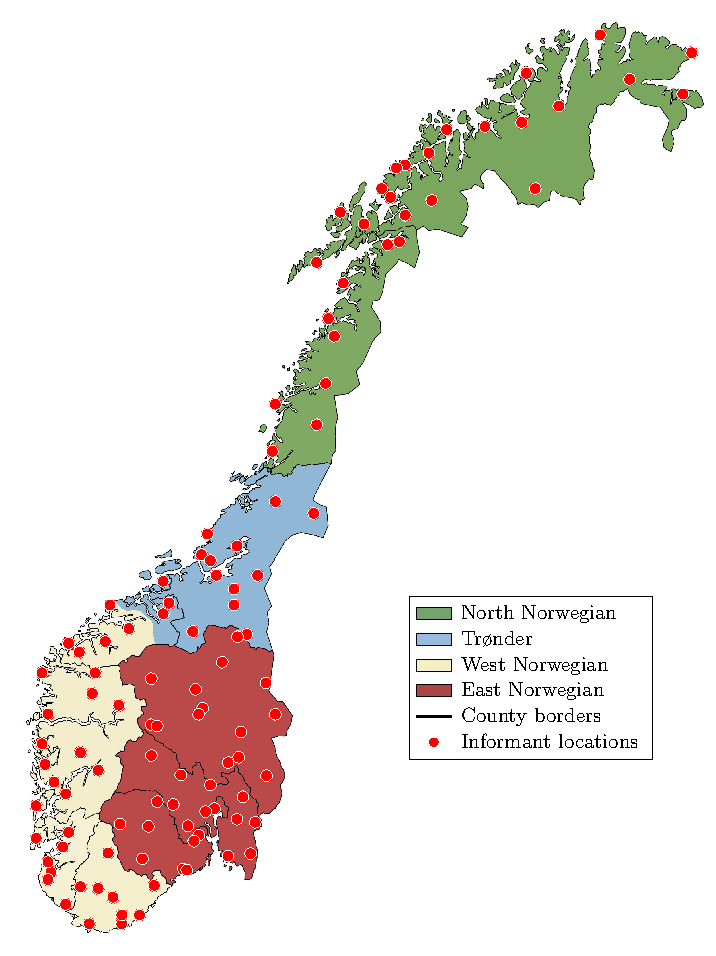
\includegraphics[width=\textwidth]{figures/3-dialects/dialect-map.pdf}
    \caption
    [Dialect areas in Norway and ScanDiaSyn informant locations]
    {Dialect areas in Norway and ScanDiaSyn informant locations.
    The division into dialect areas follows the one by \citet[p.~178]{maehlum2012dialektlandskapet}.}
    \label{fig:norway-map}
\end{figure}


This division is based on linguistic properties that I later explain in \autoref{sec:dialects-results-lingmajor}.
To some degree, such linguistic boundaries also match certain natural borders. For instance, the linguistic border between the West and East Norwegian dialect groups largely coincides with a mountain range separating the two geographic areas \cite[p.~104]{sandoey1991dialektkunnskap}.

The split into dialect groups is not entirely clear-cut, but complicated by several factors.
There is ample variation within each group, and there exist dialects that act as transition zones between the more characteristic varieties of different dialect groups \cite[p.~29]{maehlum2012dialektlandskapet}. 
Furthermore, individual regions within Northern Norway are influenced by linguistic contact in ways that do not apply to the majority of other Norwegian dialects (contact with Sámi languages and with dialects spoken by East Norwegian settlers) (\citeauthor{maehlum2012dialektlandskapet}, \citeyear{maehlum2012dialektlandskapet}, pp.~116; \citeauthor{jahr1990dialekter}, \citeyear{jahr1990dialekter}, pp.~180, 182).

% The inner part of the (former) county Troms experienced an influx of South East Norwegian settlers in the late 18th and early-to-mid 19th century \cite[p.~115]{maehlum2012dialektlandskapet}.
% To this day, the dialects spoken in this area contain dialect traits from both East and North Norwegian, to different degrees (\citeauthor{maehlum2012dialektlandskapet}, \citeyear{maehlum2012dialektlandskapet}, pp.~116; \citeauthor{jahr1990dialekter}, \citeyear{jahr1990dialekter}, pp.~180, 182).

\FloatBarrier
\section{Data}
\label{sec:tweets-data}

I work with a dataset of French tweets collected by \citet{chiril2020annotated}.%
\footnote{Available at \href{https://github.com/patriChiril/An-Annotated-Corpus-for-Sexism-Detection-in-French-Tweets}{\texttt{https://github.com/patriChiril/An-Annotated-Corpus-for-Sexism-Detection- in-French-Tweets}}.}
The data consist of French tweets that were collected in 2017 and 2018 using a list of keywords.
Such keywords include terms referring to gender or traditionally associated with one gender, gendered insults, public figures who are potential victims or perpetrators of sexism and hashtags used when recounting sexist experiences.

The tweets are annotated based on whether or not they contain sexist content.
Tweets with sexist content fall into three categories.
By far the smallest subgroup consists of \textit{directly} sexist tweets that are addressed to one or more women:

\begin{exe}
\ex Les filles qui affichent leurs corps partout et qui se disent fière, féministe ou jsp encore quelle connerie; sachez qu'on peut en être fière sans le montrer au monde entier, donc vous plaignez pas de l'image que vous renvoyez\\
`Girls who display their bodies everywhere and call themselves proud or feminist or I don't know what other nonsense; know that you can be proud of your body without showing it to the entire world, so don't complain about the image you're giving off.'

% \ex c'est vous les femmes qui sont les auteures des harcèlement par vos habilement ultra-sexy après vous dites harcèlement non ce pas juste.   \#BalanceTonPorc\\
% `It's you women who are responsible for harassment with your ultra sexy clothes and then you cry `harassment' no that's not fair. \#MeToo'

\ex Assume!  Tu fais tout pour faire le buzz et après tu pleures [EMOJI] quand on vient à moitié à poil chez Ardisson , on sait à quoi s attendre , j en ai marre de ces nanas qui n assument pas et font des histoires au nom de leur féminisme à 2 francs !\\
`Accept it! You do everything to generate buzz and then you cry [EMOJI] If you go to Ardisson['s talk show] while half-naked, you know what to expect, I'm fed up with chicks who don't stand by what they do and make a fuss in the name of their cheapo feminism!'
\end{exe}

Tweets with \textit{descriptive} sexist content are not directly addressed to anybody who would be the target of the sexist content, but describe one or more women:

\begin{exe}
\ex La cuisine pour une femme EST UN DEVOIR NATUREL comme on parlerai de droit naturel. Déjà moi je le dis tout haut: Je n'épouserais pas une femme qui ne sait pas faire la cuisine même si elle est hyper belle ou riche ou encore possède de dizaines de diplômes, juskà ce k'el l'apren\\
`For a woman, the kitchen IS A NATURAL TASK, like a law of nature. I say this loudly: I'm not gonna marry a woman who cannot cook even if she's super beautiful or rich or has dozens of diplomas until she learns to cook.'

\ex Les femmes elles sont pas crédibles dans la démarche égalité homme/femme parce qu’elles se respectent déjà pas entre elle\\
`Women aren't credible in their undertaking for equality between men and women because they don't even respect each other.'
\end{exe}

Lastly, there are tweets that \textit{report} experiences with sexism.
About 80~\% of the tweets with sexist content fall into this category; for instance:

\begin{exe}
\ex Il y a des gens (hommes) qui mettent leur numéro de tél dans leur bio pour des raisons pro Moi j'ai dû enlever mon numéro de téléphone d'un de mes CV en ligne parce qu'un élève m'a dragué par sms, et un autre mec s'en est servi alors q j'avais refusé de lui donner mon numéro\\
`There are people (men) who put their phone numbers into their bio for job reasons. I had to remove my phone number from one of my online CVs because a student tried to pick me up via SMS, and another guy used it when I had refused to give him my number.'

\ex La bonne réponse est la réponse D - 1 femme sur 5 sera victime d’un viol ou d’une tentative de viol au cours de sa vie (Source : @USAID). \#Ilesttemps de mettre fin aux \#VFS \#MoiAussi [URL]\\
`The correct answer is number D---one out of five women becomes a victim of rape or attempted rape in the course of her life (source: @USAID). \#TimesUp for putting an end to \#GenderBasedViolence \#MeToo [URL]

\ex «Si tu veux pas m'offrir ton corps, je peux le louer ?» Bordeaux — place de la Victoire \#payetashnek\\
`{``}If you don't want to offer your body to me, can I rent it?'' Bordeaux---Place de la Victoire \#payetashnek\footnote{A hashtag used for reporting sexual harassment in public spaces.}'
\end{exe}

In the version of the corpus that is available, no fine-grained distinction is made between these three subtypes of the class of tweets with \textit{sexist content} (as of writing this thesis).
The remaining tweets are labelled as \textit{non-sexist}.

The publicly available corpus does not contain the full tweets but the list of tweet IDs which can be used to retrieve the posts from Twitter.
I retrieved the tweets on December~5, 2020. 
A portion of the tweets had already been deleted, leaving about 9.700 tweets, about a third of which contain sexist content.
\autoref{tab:tweets} shows the class distribution of the original dataset and the tweets I was able to retrieve.


\begin{table}[tb]
\begin{center}
\begin{tabular}{@{}lllrrr@{}}
\toprule
\textbf{Dataset} & \multicolumn{3}{l}{\textbf{Sexist content}} & \textbf{Non-sexist} & \textbf{Total} \\
\midrule
\multirow{3}{*}{\citet{chiril2020annotated}} & \multirow{3}{*}{4,047 $\begin{dcases} \\ \\ \\ \end{dcases}$} & direct & 45 & \multirow{3}{*}{7,787} & \multirow{3}{*}{11,834} \\
 &  & descriptive & 780 &  &  \\
 &  & reporting & 3,222 &  &  \\
\midrule
My subset & \multicolumn{3}{l}{3,278} & 6,388 & 9,666 \\
\bottomrule
\end{tabular}

\end{center}
\caption{Class distribution in the Twitter corpus by \citet{chiril2020annotated} and my subset thereof.}
\label{tab:tweets}
\end{table}

It should be noted that many of the tweets are written in colloquial French and include texting abbreviations and/or spelling mistakes:


\begin{exe}
\ex 
\gll
\textbf{Tweet} Mtn y'a du sexisme envers les hommes {laissez moi} rire <URL>\\
\textbf{Standard French} \underline{Maintenant} \underline{il y a} du sexisme envers les hommes, laissez\underline{-}moi rire <URL> \\
\trans `Now there's sexism against men, I got to laugh <URL>'
\end{exe}

\begin{exe}
\ex 
\gll
\textbf{Tweet} 
Mskn tjr je m’excuse, tjr je pardonne tlm, tjr j’fais le premier pas jsuis trop conne <URL>
\\
\textbf{Standard French} 
\underline{Meskine,} \underline{toujours} je m’excuse, \underline{toujours} je pardonne \underline{tout le monde}, \underline{toujours} {\underline{je} fais} le premier pas, {\underline{je} suis} trop conne <URL>
 \\
\trans `Poor me, I always say sorry, I always forgive everybody, I always take the first stop, I'm too stupid'
\end{exe}

\begin{exe}
\ex 
\gll
\textbf{Tweet} 
Jentends un mec qui dit cest les risques du metier que natalie portman ait recu des lettres la menaçant de viol A 13 ANS et que lui il a reçu des lettres dinsultes jui MOR quel rappor
\\
\textbf{Standard French} 
J\underline{'}entends un mec qui dit c\underline{'}est les risques du m\underline{é}tier que Natalie Portman ait re\underline{ç}u des lettres la menaçant de viol A 13 ANS et que lui, il a reçu des lettres d\underline{'}insultes, \underline{je suis} MOR\underline{T(E)}, quel rappor\underline{t}
 \\
\trans `I can hear a guy who is saying that Natalie Portman receiving rape threats as a THIRTEEN YEAR OLD is a job hazard, and he's also received letters with insults, I'm DEAD, what a comparison'
\end{exe}


\subsection{General preprocessing}

I preprocess the Twitter data by replacing usernames, numbers and hashtags with \username, \numberesc{} and \hashtag, respectively.
I replace URLs with the title of the linked website when available, and remove them otherwise.
\citet{chiril2020annotated} found that replacing URLs led to better classification results.
I also normalize the punctuation by mapping different kinds of apostrophes and quotation marks to standard versions thereof.


\section{Automatic dialect disambiguation}
\label{sec:dialects-dialectometry}

A fair amount of research on \textit{dialect disambiguation}---automatically discerning between different related dialects---has been made in recent years.
Many of the results come from a range of tasks organized by the Workshop on NLP for Similar Languages, Varieties and Dialects (VarDial)  \citep{zampieri2017vardial1,zampieri2018vardial2,zampieri2019vardial3,gaman2020vardial4,chakravarthi2021vardial5}.
Participants in these tasks have used many different machine learning techniques, including recurrent or convolutional neural networks, support vector machines (SVMs), BERT, naive Bayes classifiers and ensembles thereof.

In many (though not all) of these tasks, the winning systems encode the features as bags of character- and word-level n-grams and use SVMs as the classifier (e.g. the systems by \citet{malmasi2017vardial}, \citet{bestgen2017vardial}, \citet{coltekin2018vardial} or \citet{coltekin2020vardial}).
I base my dialect classification model on this; the details are described in \autoref{sec:dialects-method}.

\section{Norwegian dialectometry}
\label{sec:norwegian-dialectometry}

While none of the VarDial tasks have focused on classifying Norwegian dialects, research in that area has been conducted.

\citet{heeringa2003norwegian} and \citet{heeringa2009measuring} cluster Norwegian dialects based on phonetic transcriptions and acoustic features and find that their results largely correspond to the findings of traditional dialectology and to speaker perceptions.
\citet[pp.~199--211]{heeringa2004measuring} clusters Norwegian dialects into groups based on acoustic differences.

\citet{gooskens2006relative} investigate to what extent prosodic, phonetic and lexical distances between Norwegian dialects correlate with perceptual distances.
\citet{beijering2008predicting} explore the correlation between phonetic distances and intelligibility ratings between Scandinavian dialects.

More recently, \cite{kaasen2020comparing} present a comparison of two different methods for quantifying dialect similarity, using a dataset that is similar to the dataset used in this thesis, in terms of how they were collected and the relatively coarse phonetic transcription style.
They show that clustering based on edit distance works well for these data and produces results that agree with the traditional dialectology, and the same applies for clusters created using neural autoencoders if the training dataset is sufficiently large.
\citeauthor{kaasen2020comparing} conclude that ``a coarse-grained transcription of
speech is sufficient to replicate known dialectal boundaries.''

\section{Method}
\label{sec:dialects-method}

I represent each preprocessed utterance as a bag of n-grams: word-level uni- and bigrams, and character-level \{1, 2, 3, 4, 5\}-grams.
All word-level n-grams are represented as a combination of their orthographic and phonetic representation.
That is, the word-level unigrams corresponding to the beginning of \hyperref[gloss:preprocessing]{Example~\ref*{gloss:preprocessing}} are: \ngram{\sos{}når/når\eos{}}, \ngram{\sos{}jeg/e\eos{}}, \ngram{\sos{}har/ha\eos{}}, and the corresponding word-level bigrams are \ngram{\sos{}når/når\sep{}jeg/e\eos{}}, \ngram{\sos{}jeg/e\sep{}har/ha\eos{}}, and so on.
The meta-tokens \ngram{\sos{}}, \ngram{\eos{}}, and \ngram{\sep{}} stand for ``start of sequence,'' ``end of sequence,'' and ``separator,'' respectively.
I also use \ngram{\sep{}} to represent the word boundary in character-level n-grams.
The word \textit{når} `when' for instance consists thus of the character bigrams \ngram{\sep{}n}, \ngram{nå}, \ngram{år}, and \ngram{r\sep{}}.

These n-grams are numerically encoded using TF-IDF (term frequency, inverse document frequency) weighting.
Only the top 5000 features (in the training data) are considered in the TF-IDF encoding step, features that appear more rarely are ignored when training and testing the model.
This encoding is done using the scikit-learn library for Python \citep{scikit-learn}.

The classifier is a support vector machine (SVM) with a linear kernel, also as implemented in scikit-learn.
The four-way classification is performed by training one one-versus-rest classifier per dialect group.

Each of these classifiers produces a prediction for a given input instance.
The confidence score for a classifier's prediction is proportional to the distance between the input instance's representation in vector space and the classifier's decision hyperplane.
The prediction probability distribution that LIME works with, $f(x)$, is the result of applying the softmax function to the classifiers' confidence scores.

\section{Results}
\label{sec:dialects-results}

The results section is structured as follows:
I first present the performance of the model and general information on the LIME-based importance scores in \autoref{sec:dialects-results-general}.
I then focus on the top 50 features per dialect group and analyze to what extent they reflect the linguistic features that are traditionally considered the most important distinctive features in Norwegian dialectology (\autoref{sec:dialects-results-lingmajor}) and other linguistics features (\autoref{sec:dialects-results-lingother}).

\subsection{General observations}
\label{sec:dialects-results-general}

I train and test the dialect classification model in ten initializations, each on a different train-test split of the dataset, and extract LIME importance scores from each of these runs.
All of the scores in this section are mean values across all ten runs.
The average model accuracy is 78.6~\% and the average (macro-averaged) F$_1$~score is 77.1~\%.

\begin{figure}[htbp]
    \centering
    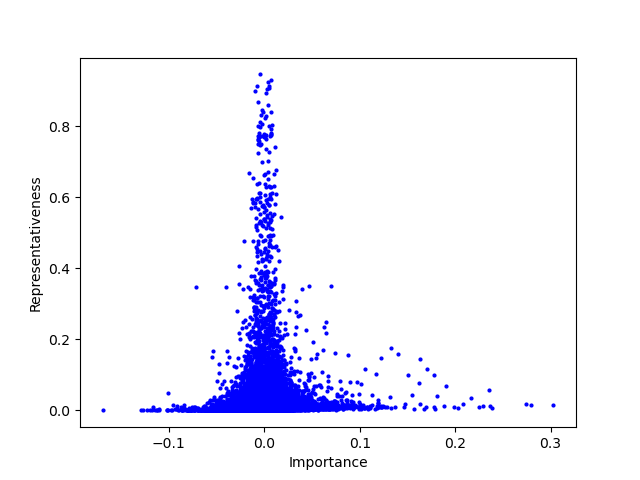
\includegraphics[width=0.9\textwidth]{figures/3-dialects/importance-rep-all-mean-unscaled.png}
    \caption
    [Representativeness values by LIME score for dialect classification]
    {Representativeness values by LIME importance score per feature-label combination.}
    \label{fig:imp-rep}
\end{figure}
\begin{figure}[htbp]
    \centering
    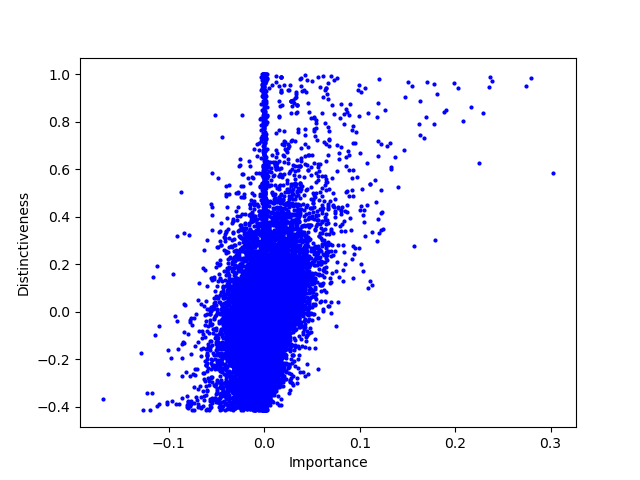
\includegraphics[width=0.9\textwidth]{figures/3-dialects/importance-dist-all-mean-unscaled.png}
    \caption
    [Distinctiveness values by LIME score for dialect classification]
    {Distinctiveness values by LIME importance score per feature-label combination.}
    \label{fig:imp-dist}
\end{figure}

Importance values range between -0.17 and +0.30, with no significant distribution differences for the different dialect groups.
There is only a marginal correlation between a feature's importance score for a label and the corresponding representativeness value, i.e. in which proportion of the instances with that label it is present.
This is not very surprising, as most features with high representativeness scores are representative of \textit{all} dialect groups.
This is for instance the case with almost all character unigrams.
The correlation coefficient (Pearson's \textit{R}) between importance and representativeness is between 0.03 and 0.05 for the different dialect groups,
and this is also illustrated in \autoref{fig:imp-rep}.
However, the importance score does correlate with the distinctiveness score, that is, features with higher importance scores for a label tend to mostly occur in utterances with that gold-standard label (\autoref{fig:imp-dist}).
The correlation coefficient between importance and distinctiveness is between 0.37 and 0.41 for the different dialect groups.


\begin{table}[htbp]
    \centering
\begin{tabular}{lrlrlrlrl}
\toprule
\textbf{Word} & \multicolumn{2}{l}{\begin{tabular}[c]{@{}l@{}}\textbf{West} (actual\\\& predicted label)\end{tabular}} & \multicolumn{2}{l}{\textbf{East}} & \multicolumn{2}{l}{\textbf{Trønder}} & \multicolumn{2}{l}{\textbf{North}} \\
\midrule
\textit{ja} /ja/ {\smaller``yes''}  &  & &  &  &  &  &  &  \\
\multirow{2}{*}{\begin{tabular}[c]{@{}l@{}}\textit{da} /då/ \\ \phantom{~~}{\smaller``then''} \end{tabular}} & \cellcolor[HTML]{72C69D}0.17  & då\sep{}& {\cellcolor[HTML]{F5CDCA}-0.07} & då\sep{} & {\cellcolor[HTML]{F5CECB}-0.07} & \multicolumn{2}{l}{då\sep{}}  &  \\
 & \cellcolor[HTML]{F7D6D3}-0.06 & \sep{}då &  &  &  &  &  &  \\
\textit{vi} /me/ {\smaller``we''} & \cellcolor[HTML]{A1D9BE}0.11  & \multicolumn{2}{l}{{\ngram{\sos{}vi/me\eos{}}}}  &  &  &  & {\cellcolor[HTML]{F5CBC7}-0.08} & {\ngram{\sos{}vi/me\eos{}}}  \\
\multirow{2}{*}{\begin{tabular}[c]{@{}l@{}}\textit{har} /he/\\ \phantom{~~}{\smaller``have.\textsc{pres}''} \end{tabular}} & \cellcolor[HTML]{BAE3CF}0.08 & he\sep{} & {\cellcolor[HTML]{F7D6D4}-0.06} & he\sep{} &  &  &  &  \\
 & \cellcolor[HTML]{D2EDE0}0.05 & \multicolumn{2}{l}{\sos{}har/he\eos{}} &  &  &  &  &  \\
\multirow{2}{*}{\begin{tabular}[c]{@{}l@{}}\textit{de} /di/ \\ \phantom{~~} {\smaller``the.\textsc{pl}''} \end{tabular}}& \cellcolor[HTML]{D1EDDF}0.06  & \sep{}di&  &  &  &  &  &  \\
\\
\multicolumn{3}{l}{\textit{siste} /sisste/ {\smaller``last.\textsc{def}''}}  & &  &  &  &  &  \\
\multicolumn{3}{l}{\textit{årene} /åran/ {\smaller``years.\textsc{def}''}}  & &  &  &  &  &  \\
\multirow{2}{*}{\begin{tabular}[c]{@{}l@{}}\textit{nå} /nå/\\ \phantom{~~}{\smaller``now''} \end{tabular}}& \cellcolor[HTML]{F1B7B3}-0.11 &  \sep{}nå & &  &  &  &  &  \\
 & \cellcolor[HTML]{BFE5D2}0.08 & nå\sep{} &  &  &  &  &  &  \\
\textit{så} /så/ {\smaller``so''} &  & &  &  &  &  &  &  \\
\multirow{2}{*}{\begin{tabular}[c]{@{}l@{}}\textit{har} /he/\\ \phantom{~~}{\smaller``have.\textsc{pres}''} \end{tabular}} &  \cellcolor[HTML]{D2EDE0}0.05 &\multicolumn{2}{l}{\sos{}har/he\eos{}}  &  &  &  &  &  \\
 & \cellcolor[HTML]{BAE3CF}0.08 & he\sep{} &  &  &  &  &  &  \\
\textit{vi} /mi/ {\smaller``we''} & \cellcolor[HTML]{94D4B5}0.13 & {\smaller\ngram{\sos{}vi/mi\eos{}}} & {\cellcolor[HTML]{F7D9D7}-0.06}& \multicolumn{3}{l}{{\ngram{\sos{}vi/mi\eos{}}}}  & {\cellcolor[HTML]{F7D5D3}-0.06}& {\ngram{\sos{}vi/mi\eos{}}}  \\
& \cellcolor[HTML]{AFDFC8}0.10  & \sep{}mi &  {\cellcolor[HTML]{F4C7C3}-0.09} &\sep{}mi &  &  &  &  \\
\multicolumn{3}{l}{\textit{vært} /værrt/ {\smaller``been''}} &  &  &  &  &  &  \\
\multicolumn{3}{l}{\textit{heldige} /helldi/ {\smaller``lucky.\textsc{pl}''}}  & &  &  &  &  &  \\
\bottomrule
\end{tabular}
    \caption
    [LIME scores for a sample utterance]
    {LIME scores for a (correctly predicted) West Norwegian utterance.
    Features with importance scores between -0.05 and +0.05 are omitted to preserve space.
    No word bigrams have importance scores that lie below/above that threshold.}
    \label{tab:sample-sentence}
\end{table}

\autoref{tab:sample-sentence} shows the importance scores for each label for a sample sentence, the West Norwegian utterance \textit{ja da [.] vi har [---] de siste årene nå så har vi vært heldige}
/ja då me he di sisste åran nå så he mi værrt helldi/
``Yes. We have---the past few years now, we've been lucky.''
(Note that these are the LIME scores for this specific utterance and not the global importance scores.)
This utterance is represented by 100 features, the vast majority of which have LIME scores that are close to zero.
This utterance was correctly predicted as West Norwegian and that prediction is also reflected by the distribution of importance scores: in this case, only the West Norwegian label is associated with (more than marginally) positive importance scores, while the importance scores for the other combinations of features and labels tend to be close to zero (signifying that a feature is insignificant for predicting the given label) or negative (indicating that the presence of the feature lowers the likelihood of the given label being predicted).
It should be noted that importance scores can seem contradictory: in the sample sentence, the words \textit{da} /d\aa/ and \textit{n\aa} /n\aa/ are represented by a feature \ngram{\sep{}d\aa} (\ngram{\sep{}n\aa}) ``/d\aa/ (/n\aa/) is a prefix (or full word)'' and another feature \ngram{d\aa\sep{}} (\ngram{d\aa\sep{}}) ``/d\aa/ (/n\aa/) is a suffix (or full word),'' where the former receives a negative importance score and the latter a positive one.


\begin{figure}[htbp]
    \centering
    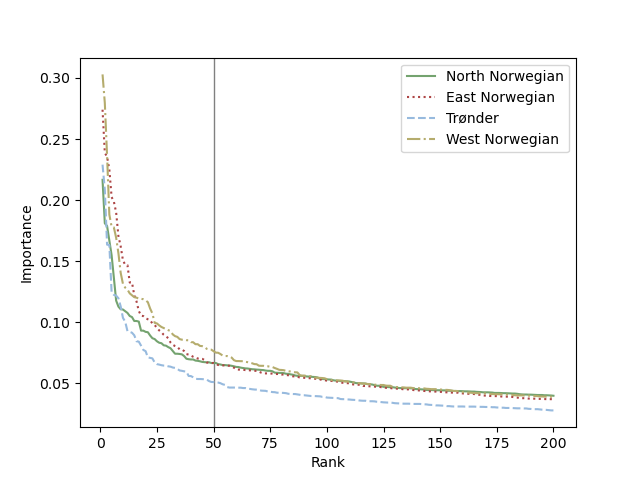
\includegraphics[width=0.9\textwidth]{figures/3-dialects/importance-rank-all-mean-unscaled-50.png}
    \caption
    [Importance score by rank and dialect group]
    {Importance score by rank and dialect group.}
    \label{fig:imp-rank}
\end{figure}
\begin{figure}[htbp]
    \centering
    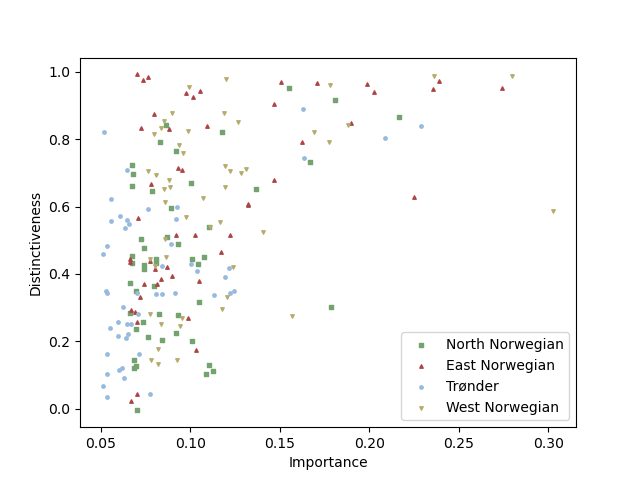
\includegraphics[width=0.9\textwidth]{figures/3-dialects/importance-dist-all-mean-unscaled-50.png}
    \caption[Distinctiveness by LIME score for the 50 highest-ranking features per dialect group]
    {Distinctiveness by importance score for the 50 highest-ranking features per label.}
    \label{fig:imp-dist50}
\end{figure}

In the following two sections, I qualitatively examine the 50 features with the highest importance scores per predicted label.
I chose this threshold to strike a balance between only analyzing features with relatively high importance scores and having a sizable selection of features to analyze.
\autoref{fig:imp-rank} shows the importance scores for the features included in the analysis as well as the scores of the succeeding ranks.
The selected features show a correlation between importance score and distinctiveness, as illustrated in \autoref{fig:imp-dist50}.
The following analysis includes the 50 features per class that have the highest importance scores.\footnote{%
I share tables with the 200 most important features per dialect group at \url{https://github.com/verenablaschke/ma-thesis/tree/main/models/dialects}.
}
These features tend to mostly include variants of high-frequency words, as well as some common short sequences of phonemes.
Only one of those high-importance features is clearly about a conversation topic (rather than lexical choice or pronunciation): the trigram \ngram{ami} in North Norwegian utterances, which usually appears in the word \textit{samisk} `Sámi' and inflected versions thereof.
This is not a surprise as most Sámi cultural centres are located in the Northern part of the country.




\subsection{Major linguistic features}
\label{sec:dialects-results-lingmajor}

In this section, I introduce the linguistic characteristics that are typically discussed in Norwegian dialectology and point out which of these can be found in the ScanDiaSyn data and whether they are considered as important by LIME.

Different dialectologists use somewhat different sets of linguistic features to characterize the different dialect groups.
In this section, I present a summary of those features that are regularly brought up in the literature on Norwegian dialectology.

\citet[pp.~113--115]{sandoey1991dialektkunnskap} uses the features detailed in \autoref{sec:dialects-features-inffem} to discern between twelve dialect groups (that are subgroups of the four groups I use in this thesis).
\citet[pp.~32--42]{maehlum2012dialektlandskapet} base their classification on the features in \autoref{sec:dialects-features-inffem}, \autoref{sec:dialects-prosody}, and \autoref{sec:dialects-features-tjukkl}.
These are also the features considered most important by \citet{kaasen2020comparing}.


\subsubsection{Infinitive endings and endings of feminine nouns}
\label{sec:dialects-features-inffem}

One prominently discussed group of features is concerned with the different ways in which word-final vowels of infinitives or certain feminine nouns have changed.
The following explanation summarizes the overviews by 
\citet[pp.~33--35]{maehlum2012dialektlandskapet} and \citet[pp.~113--114]{sandoey1991dialektkunnskap}.

In Old West Norse, infinitive forms of verbs with more than one syllable ended in /-a/, as did the so-called `weak' feminine nouns (that is, feminine nouns ending in a vowel sound rather than a consonant).
The following types of dialects have emerged with regard to how this ending has (or has not) changed:
\begin{itemize}
    \item \textit{A-mål} `a-speech': In these dialects, all such words still end in /-a/ (or another non-schwa vowel).
    \item \textit{E-mål} `e-speech': The endings of both infinitives and weak feminine nouns were reduced to a schwa.
    \item Apocope: Both infinitives and weak feminine nouns have undergone apocope.
    \item \textit{E/a-mål} `e/a-speech': Only the infinitive endings were reduced to a schwa, weak feminine nouns still end in /-a/ (or another non-schwa vowel).
    \item \textit{Jamvektsmål} `balance-speech': Whether or not the final vowel was reduced or not depends on the length of the root of the word. Only infinitives and weak feminine nouns with short roots retained endings with full endings, whereas words with roots whose rhyme contained a long vowel and/or multiple consonants now end in /-\textschwa{}/.
    \item \textit{Jamvekt} with apocope: These dialects behave like the previous group, but the final vowel of a word with a long root was dropped.
\end{itemize}

For classifying to which of the major dialect groups a doculect belongs, \textit{jamvekt} and apocope are often considered the most distinctive indicators \cite[pp.~32--42]{maehlum2012dialektlandskapet}.
East Norwegian dialects fall into the \textit{jamvekt} group (with /-\textschwa{}/) \cite[p.~46]{maehlum2012dialektlandskapet}.
Tr{\o}nder dialects exhibit \textit{jamvekt} with apocope (p.~76), and West Norwegian dialects are instances of \textit{a-mål} and \textit{e-mål} (p.~90).
The different North Norwegian dialects fall into all of the listed groups except for either of the \textit{jamvekt} types (pp.~106--107).

All of the phenomena listed in this section can be found in the data, albeit not overtly encoded.
However, they can at least be partially found when inspecting common infinitive forms in the data:
The by far most common (multisyllabic) infinitives in the ScanDiaSyn data are \textit{(å) være} `(to) be,' \textit{(å) gjøre} `(to) do,' and \textit{(å) komme} `(to) come.'
All three verbs are in the group of verbs whose ending is \textit{not} reduced in \textit{jamvekt} dialects \cite[cf.][p.~84]{hanssen2010dialekter}; therefore knowing the infinitive forms of these verbs for a given dialect is \textit{not} sufficient for figuring out exactly which suffix group the dialect belongs to, although it can be used to narrow down the options, as shown in \autoref{tab:jamvekt}.

\begin{table}[htbp]
    \centering
\begin{tabular}{llll}
\toprule
\textbf{Type} & \begin{tabular}[c]{@{}l@{}} \textbf{(å) være}\\ `(to) be' \end{tabular} & \begin{tabular}[c]{@{}l@{}} \textbf{(å) gjøre} \\`(to) do' \end{tabular} & \begin{tabular}[c]{@{}l@{}} \textbf{(å) komme}\\`(to) come' \end{tabular} \\\midrule
A-mål, jamvekt & væra, vårrå, værra & jørra, jøra, jera & kåmma, kåmmå \\
E-mål, e/a-mål & være & jøre, jære & kåmme, kåme \\
Apocope & vær, væ & jør, jær, jørr & kåmm \\\bottomrule
\end{tabular}

% være (849), vær (734), væra (305), væ (207), vårrå (196), værra (191), vera (143), vara (106), ver (93), va (79), vere (78), ve (58), var (56), varra (56), værr (42), vørrå (40), vørå (38), vørr (28), verra (27), vare (26), vårr (26), vør (19), værre (18), vårå (14), varr (11), vår (11), våre (8), vårre (8), vøre (6), væær (5), vårra (4), vørre (3), vø (3), vå (3), vørra (3), vææ (2), vøra (2), våra (1), varre (1), bea (1), vi (1), vørø (1), væe (1), vore (1), varrå (1), varran (1), værrt (1), viere (1)

% jør (299), jøre (260), jær (230), jørra (110), jøra (108), jera (100), jære (70), jæra (67), jørr (59), jer (52), jørrå (43), jærra (29), jere (20), jø (13), jerra (12), jøør (9), jørå (6), jørre (4), jærre (3), jærr (3), jæ (3), gjøre (3), gjør (2), jerran (2), jærn (1), jøɽe (1), jårra (1), jærran (1), jerrå (1), jærrå (1), jår (1), gøre (1), gjøra (1), gjørra (1), øre (1), jøe (1)

% kåmme (385), kåmma (220), kåmm (195), kåmmå (77), kåme (30), kåma (25), komme (13), komm (12), komma (11), çæmm (5), koma (1), kåmmi (1), çem (1), kommi (1), çemm (1), kømmi (1), kåm (1), kåmmer (1), kommå (1)

    \caption
    [Infinitive forms of the most common verbs in ScanDiaSyn]
    {The most common infinitive forms of the three most common (non-monosyllabic) verbs in the ScanDiaSyn corpus, grouped by the type of ending.
    The examples in this table are by no means exhaustive.
    The \textit{jamvekt} subgroup here includes both dialects with and without apocope.}
    \label{tab:jamvekt}
\end{table}
\begin{table}[htbp]
    \centering
\begin{tabular}{llrrrl}
\toprule
\textbf{Group} & \textbf{Feature} & {\textbf{Imp.}} & {\textbf{Rep.}} & {\textbf{Dist.}} & \textbf{Context (bokm\aa{}l/pron.)} \\\midrule
East & \ngram{æra\sep{}} & 0.08 & 0.01 & 0.44 &
{\begin{tabular}[c]{@{}l@{}}være/væra(0.7)	`(to) be'\\gjøre/jæra(0.1) `(to) do'\end{tabular}}
\\\midrule
\multirow{2}{*}{Trø.}  & \ngram{rrå} & 0.09 & 0.02 & 0.56 & {\begin{tabular}[c]{@{}l@{}}være/vårrå(0.7) `(to) be'\\	fare/fårrå(0.1) `(to) drive'\end{tabular}} \\
 & \ngram{rra\sep{}} & 0.05 & 0.02 & 0.24 & {\begin{tabular}[c]{@{}l@{}} være/værra(0.2) `(to) be'\\  gjøre/jørra(0.2) `(to) do'\end{tabular}}	\\\bottomrule
\end{tabular}

    \caption
    [Infinitive endings in the top 50 most important features per dialect group]
    {Features encoding infinitive endings that are among the top 50 most important features per dialect group.
    The context column contains the most common token-level context for character n-grams (numbers in parentheses indicate the proportion of context tokens a character n-gram comes from).}
    \label{tab:results-inf}
\end{table}

Versions of \textit{være} and \textit{gjøre} are represented among the features with high importance scores for instances predicted as East Norwegian or Trønder: \ngram{\ae{}ra\sep} in East Norwegian and \ngram{rr\aa} and \ngram{rra\sep} in Tr\o{}nder; all indicating full vowel endings, as expected.
All of these features represent both \textit{være} and \textit{gjøre} at the same time (and in one case, the verb \textit{(å) fare} `(to) drive' as well).
None of the highest-ranking features include versions of \textit{komme} despite it also appearing frequently in the data (but there are also no other frequent verbs in the dataset whose stem ends in \textit{-mm}).

No feminine nouns (or features that clearly encode the ending of a feminine noun) are among any dialect group's top 50 labels.
However, even the most frequently appearing weak feminine nouns (\textit{klasse} `class,' \textit{uke} `week,' and \textit{hytte} `hut') occur significantly less often than the most common verbs.

\subsubsection{Prosody}
\label{sec:dialects-prosody}

A second distinctive feature is the realization of the two tonemes that exist within the context of Norwegian pitch accent.
When a word has accent~1, speakers of East Norwegian and Trønder begin with a low pitch whereas West and North Norwegian dialect speakers tend to begin with a high pitch \cite[p.~37]{maehlum2012dialektlandskapet}.
An experiment by \citet{gooskens2005norwegians} shows that intonation information plays a significant role when Norwegians are asked to determine where a dialect speaker is from.
This is also confirmed by \citet{ommeren2019tonefall}.
Toneme information is \textit{not} encoded in the ScanDiaSyn dataset.

However, \citet[pp.~36--37]{maehlum2012dialektlandskapet} mention another prosodic feature that correlates with the toneme patterns: word-level stress in particle verbs and in many Greek and Romance loanwords.
Generally, the last syllable of such a loanword (and the particle in a particle verb) are stressed in North and West Norwegian, whereas the first syllable (and the verb) are stressed in East Norwegian and Trønder (\citeauthor{hanssen2010dialekter}, \citeyear{hanssen2010dialekter}, pp.~58--59; \citeauthor{maehlum2012dialektlandskapet}, \citeyear{maehlum2012dialektlandskapet}, pp.~37, 78).
While the stress pattern in particle verbs is not always overtly represented in ScanDiaSyn,%
\footnote{It is only transcribed when the stress lies on the verb and the stressed syllable within the verb contains a short vowel.}
it is encoded in some loanword transcriptions, such as pronunciations of \textit{spesiel} `special,' which is transcribed as either \ngram{spessiel} (with stress on the first syllable) or \ngram{spesiell} (with stress on the second syllable).
None of the top 50 features encode stress information.
The highest-ranking feature to do so is \ngram{ssi} in Trønder (rank 59 with a mean importance score of 0.05), which most often appears in phonetic transcriptions of the words \textit{spesielt} `special, especially' and \textit{musikk} `music.'

\subsubsection{Retroflex flap}
\label{sec:dialects-features-tjukkl}

\begin{table}[htbp]
    \begin{tabular}{llrrrl}
\toprule
\textbf{Group} & \textbf{Feature} & \textbf{Imp.} &{\textbf{Rep.}} & {\textbf{Dist.}} & \textbf{Context (bokmål/pron.)} \\\midrule
\multirow{3}{*}{East} & \ngram{ø\textrtailr{}\textrtailr{}} & 0.15 & 0.01 & 0.68 & {folk/fø\textrtailr{}\textrtailr{}k(0.2) `people'}\\
& \ngram{\sep{}b\textrtailr{}e} & 0.11 & 0.01 & 0.84 & ble/b\textrtailr{}e(0.8) `became'\\
& \ngram{\textrtailr{}æi} & 0.08 & 0.01 & 0.87 & blei/b\textrtailr{}æi(0.7) `became'\\
 & \ngram{\sep{}o\textrtailr{}} & 0.07 & 0.00 & 0.56 & {ord/o\textrtailr{}(0.9) `word'}\\\midrule
\multirow{5}{*}{Tr\o.} & \ngram{e\textrtailr{}\sep{}} & 0.06 & 0.02 & 0.62 & {vel/ve\textrtailr{}(0.6) `well'} \\
& \ngram{\sep{}væ\textrtailr{}} & 0.06 & 0.02 & 0.54 & {vel/væ\textrtailr{}(1.0) `well'} \\
& \ngram{\sep{}ve\textrtailr{}} & 0.06 & 0.01 & 0.71 & {vel/ve\textrtailr{}(1.0) `well'} \\
& \ngram{ø\textrtailr{}} & 0.06 & 0.03 & 0.25 & {sjøl/\textrtails{}ø\textrtailr{}(0.4)  `self'} \\
& \ngram{æ\textrtailr{}\sep{}} & 0.05 & 0.02 & 0.48 & {vel/væ\textrtailr{}(0.7) `well'} \\\bottomrule
\end{tabular}

    \caption{Features with high importance values that contain /{\textrtailr}/.}
    \label{tab:tjukk-l}
\end{table}

Another important feature is the presence or absence of the retroflex flap.
In many dialects, the Old Norse phoneme /l/ changed to /{\textrtailr}/ in many phonological environments, and often, Old Norse /r{\dh}/ also changed to /{\textrtailr}/ (instead of /r/) \cite[p.~185]{sandoey1991dialektkunnskap}.


These changes are characteristic of East Norwegian and Tr{\o}nder dialects, whereas West Norwegian dialects do not have this consonant, and the North Norwegian dialect area contains dialects with and without /{\textrtailr}/ \cite[pp.~36, 184]{maehlum2012dialektlandskapet}.

The East Norwegian and Trønder dialects contain several high-ranking features that include /{\textrtailr}/ (\autoref{tab:tjukk-l}).
In most cases, these features are character-level n-grams that only appear in one or a few words in the corpus at large, although these words tend to be quite common.
However, the unigram \ngram{\textrtailr} achieves a relatively high ranking among the East Norwegian features (despite not making it past the rank threshold): it is at rank 56 with an importance score of 0.06.

\subsection{Other linguistic features}
\label{sec:dialects-results-lingother}

The previously mentioned features are by far not the only features included in classifications and descriptions of Norwegian dialects.
This section presents some of the other linguistic features with high importance scores that are often discussed in Norwegian dialectology, despite not always being considered the most essential for deciding where the borders between the dialect areas should be drawn.

\subsubsection{Personal pronouns}
\label{sec:dialects-results-pronouns}

\begin{table}[htbp]
    \centering
\begin{tabular}{lllrrrl}
\toprule
\textbf{Pron.} & \textbf{Group} & \textbf{Feature} & \textbf{Imp.} & \textbf{Rep.} & \textbf{Dist.} & \begin{tabular}[c]{@{}l@{}}\textbf{Context}\\\textbf{(bokmål/pron.)}\end{tabular} \\\midrule
\multirow{8}{*}{\begin{tabular}[c]{@{}l@{}}\textsc{1.sg}\\\textsc{nom}\end{tabular}}
& {North} & \ngram{\sos{}jeg/æ\eos{}} & 0.07 & 0.16 & 0.43 &  \\
\cmidrule{2-7}
 & \multirow{4}{*}{East} & \ngram{\sos{}jeg/je\eos{}} & 0.19 & 0.07 & 0.85 &  \\
 &  & \ngram{\sos{}jeg/jæ\eos{}} & 0.17 & 0.12 & 0.97 &  \\
 &  & \ngram{\sep{}jæi} & 0.15 & 0.02 & 0.91 & \context{jeg/jæi(1.0)} \\
 &  & \ngram{jæ\sep{}} & 0.11 & 0.12 & 0.94 & \context{jeg/jæ(1.0)} \\
\cmidrule{2-7}
 & \multirow{3}{*}{West} & \ngram{\sos{}jeg/i\eos{}} & 0.30 & 0.02 & 0.59 &  \\
 &  & \ngram{\sos{}jeg/ei\eos{}} & 0.17 & 0.01 & 0.82 &  \\
 &  & \ngram{eg\sep{}} & 0.09 & 0.16 & 0.68 & \context{jeg/eg(0.9)} \\ 
\midrule
 \multirow{2}{*}{\begin{tabular}[c]{@{}l@{}}\textsc{1.sg}\\\textsc{acc}\end{tabular}} & Tr\o. & \ngram{\sos{}meg/mæ\eos{}}  & 0.06 & 0.02 & 0.11 &  \\\cmidrule{2-7}
 & East & \ngram{mæi\sep{}}  & 0.08 & 0.01 & 0.67 & \context{meg/mæi(0.9)} \\\midrule
\multirow{4}{*}{\begin{tabular}[c]{@{}l@{}}\textsc{1.pl}\\\textsc{nom}\end{tabular}} 
 & Tr\o. & \ngram{\sos{}vi/åss\eos{}} & 0.10 & 0.02 & 0.43 &  \\\cmidrule{2-7}
 & \multirow{2}{*}{West} & \ngram{\sos{}vi/mi\eos{}} & 0.12 & 0.02 & 0.66 &  \\
 &  & \ngram{\sos{}vi/me\eos{}}  & 0.10 & 0.08 & 0.57 &  \\
\bottomrule
\end{tabular}
    \caption
    [First person pronouns in the top 50 most important features per dialect group]
    {First person pronouns in the top 50 most important features per dialect group.
    The middle columns contain importance, representativeness and distinctiveness scores.
    The context column lists the most frequent word in which each character n-gram appears (along with the relative frequency of this word being the origin).}
    \label{tab:pronouns-1}
\end{table}

There is also ample variation in the variants of personal pronouns. 
The first person singular pronoun \textit{jeg} is pronounced /e(g)/ or /{\ae}g/ in large parts of the country, but with an initial /j-/ (/je/ or /j{\ae}(i)/) in much of the East Norwegian area
\cite[pp.~22--23]{jahr1990dialekter}.
In parts of West Norway and Trøndelag, the variant /i/ is also in use \cite[pp.~22--23]{jahr1990dialekter}.
Apart from the geographic distribution of /i/, the literature generally does not show such a subdivision and tends to lump together the forms without /j-/ in the remaining regions.
\autoref{tab:pronouns-1} shows the first personal singular forms that rank among each dialect group's 50 highest-scoring LIME features.
These results clearly show the presence of an initial glide in East Norwegian \textsc{1.sg} forms.
The North Norwegian form with the highest importance score is /\ae/. 
While it is not the only form used in that dialect group, \citet[p.~36]{jahr1996nordnorske} already remarked upon its spreading popularity several decades ago.
Additionally, the results highlight several West Norwegian pronoun variants: \ngram{\sos{}jeg/i\eos{}}, \ngram{\sos{}jeg/ei\eos{}} and \ngram{eg\sep{}}.
While these are generally not used to characterize the entire West Nowegian dialect group, they are characteristic for several dialects within that group \citet[pp.~71, 74, 76, 79]{sandoey1996vestlandet}.
Despite being a lot less commonly discussed by dialectologists than the first person singular nominative pronoun, two versions of the accusative form also receive high importance scores: Trønder /mæ/ and East Norwegian /mæi/.

\textit{Vi}, the first person plural pronoun, is replaced by /me/ or /mi/ in many West Norwegian and some East Norwegian dialects, and by /{\aa}ss/ in some other East, West and Trønder Norwegian dialects \cite[p.~183]{maehlum2012dialektlandskapet}.
\autoref{tab:pronouns-1} also shows the first person plural forms that are among the most important features, as determined by LIME.
These clearly reflect the West Norwegian tendency to use /me/ or /mi/.
The results also include Tr\o{}nder /åss/, which---while also attested in other dialect groups---is more characteristic of Tr\o{}nder in the ScanDiaSyn data (about half of the occurrences of \ngram{\sos{}vi/\aa{}ss\eos{}} appear in just 14~\% of the data).

\begin{table}[htbp]
    \centering
\begin{tabular}{lllrrrl}
\toprule
\textbf{Pron.} & \textbf{Group} & \textbf{Feature}  & \textbf{Imp.} & \textbf{Rep.} & \textbf{Dist.} &  \begin{tabular}[c]{@{}l@{}}\textbf{Context}\\\textbf{(bokmål/pron.)}\end{tabular} \\\midrule
\multirow{5}{*}{\begin{tabular}[c]{@{}l@{}}\textsc{2.sg}\\\textsc{nom}\end{tabular}} & \multirow{2}{*}{East} & {\smaller\ngram{\sos{}vet/vett\sep{}du/du\eos{}}} & 0.08 & 0.01 & 0.38 &  \\
 &  & \ngram{\sep{}ru} & 0.08 & 0.03 & 0.41 & du/ru(0.8) \\
 \cmidrule{2-7}
 & \multirow{2}{*}{Trø.} & {\smaller\ngram{\sos{}vet/vet\sep{}du/du\eos{}}} & 0.09 & 0.03 & 0.34 &  \\
 && \ngram{\sos{}du/u\eos} &	0.06 &	0.01&0.22 \\\cmidrule{2-7}
 & West & \ngram{do\sep{}} & 0.13 & 0.01 & 0.70 & du/do(0.9) \\\midrule
\begin{tabular}[c]{@{}l@{}}\textsc{2.sg}\\\textsc{acc}\end{tabular} & Trø. & \ngram{\sos{}deg/dæ\eos{}} & 0.06 & 0.01 & 0.12 &  \\
\midrule
\textsc{2.pl} & {North} & \ngram{dåkke} & 0.07 & 0.01 & 0.50 & dere/dåkker(0.7) \\
\bottomrule
\end{tabular}
    \caption[Second person pronouns in the top 50 most important features per dialect group]
    {Second person pronouns in the top 50 most important features per dialect group.
    The middle columns contain importance, representativeness and distinctiveness scores.
    The context column lists the most frequent word in which each character n-gram appears (along with the relative frequency of this word being the origin).}
    \label{tab:pronouns-2}
\end{table}


The second person singular (nominative) pronoun is not commonly presented as a particularly important feature for distinguishing between dialect groups.
In most dialects, it is /du/, although (when unstressed) it is reduced to /ru/ in some East Norwegian dialects (\citeauthor{haarstad2013spraak}, \citeyear{haarstad2013spraak}, p.~88; \citeauthor{endresen1990vikvaersk}, \citeyear{endresen1990vikvaersk}, p.~97; \citeauthor{wiggen1990oslo}, \citeyear{wiggen1990oslo}, p.~184).
The high-ranking features include East Norwegian /ru/ as well as a West Norwegian form /do/.
The latter does in fact most commonly appear in West Norway in the ScanDiaSyn data (although /du/ is nevertheless the most frequent pronunciation in that part of the country) but it is not remarked upon in the descriptions of West Norwegian dialects by \citet{sandoey1996vestlandet}, \citet[pp.~168, 176, 185]{hanssen2010dialekter} or \citet[p.~91]{maehlum2012dialektlandskapet}.
Two word bigrams with different variations of \textit{vet du} `you know; do you know' also have high importance scores among the East Norwegian and Tr\o{}nder features, but both include the common form /du/ and only differ in the vowel length of /vet(t)/.
Tr\o{}nder also has the high-importance variant /u/, which is not commonly pointed out in descriptions of the dialect group.
The accusative form \textit{deg} usually also goes unremarked in dialectologist literature, but the Trønder pronunciation /d\ae/ has a relatively high importance score (similarly to the Trønder \textsc{1.sg.acc} form /m\ae/).

Different dialects use different lexemes for second person plural pronouns.
In East and West Norwegian areas, variants of /di, de/ (\textsc{nom}) and /dere/ or /dVkk, dVkkV(r/n)/ (\textsc{acc} or regardless of case) prevail \citep[pp.~80--86]{papazian2008dedykkdere}.
Speakers of Trønder dialects use /di, de/ (\textsc{nom}) and /dåkk/ (\textsc{acc} or regardless of case) \citep[p.~86]{papazian2008dedykkdere}, whereas North Norwegian dialects do not make any case distinction and use forms resembling /dåkk(er)/ \citep[p.~87]{papazian2008dedykkdere}.
Of these forms, only the North Norwegian /d\aa{}kker/ appears in the top 50 features per dialect group (see \autoref{tab:pronouns-2}).


\begin{table}[htbp]
    \centering
\begin{tabular}{lllrrrl}
\toprule
\textbf{Pron.} & \textbf{Group} & \textbf{Feature} & \textbf{Imp.} & \textbf{Rep.} & \textbf{Spec.} & \begin{tabular}[c]{@{}l@{}}\textbf{Context}\\\textbf{(bokmål/pron.)}\end{tabular} \\\midrule
\multirow{2}{*}{\textsc{3.sg}} & \multirow{2}{*}{North} & \ngram{\sos{}hun/o\eos{}} & 0.09 & 0.01 & 0.28 &  \\
 &  & \ngram{ho\sep{}} & 0.08 & 0.04 & 0.21 & hun/ho(0.9) \\
 \midrule
\multirow{7}{*}{\textsc{3.pl}} 
 & \multirow{3}{*}{East} & \ngram{\sep{}ræi} & 0.10 & 0.01 & 0.17 & de/ræi(0.4) \\
 &  & \ngram{dømm\sep{}} & 0.07 & 0.02 & 0.97 & de/dømm(0.8)\\
 &  & \ngram{ømm\sep{}} & 0.07 & 0.02 & 0.83 & de/dømm(0.6) \\
\cmidrule{2-7}
 & {Tr\o.} & \ngram{\sep{}æmm} & 0.16 & 0.02 & 0.74 & de/æmm(0.9) \\
\cmidrule{2-7}
 & \multirow{4}{*}{West} & \ngram{\sos{}de/dei\eos{}} & 0.09 & 0.01 & 0.85 &  \\
 &  & \ngram{\sos{}de/dæi\eos{}} & 0.08 & 0.06 & 0.69 &  \\
 &  & \ngram{\sep{}dei} & 0.08 & 0.01 & 0.70 & de/dei(0.9)\\
\bottomrule
\end{tabular}
    \caption[Third person pronouns in the top 50 most important features per dialect group]
    {Third person pronouns in the top 50 most important features per dialect group.
    The middle columns contain importance, representativeness and distinctiveness scores.
    The context column lists the most frequent word in which each character n-gram appears (along with the relative frequency of this word being the origin).}
    \label{tab:pronouns-3}
\end{table}

The most common variant of the third person feminine singular pronoun is /ho/, although /hu(n)/ is also common in East Norwegian and /hon/ in parts of West Norway \citep[p.~110]{hanssen2010dialekter}.
Only the North Norwegian dialect group contains features encoding this pronoun in its top 50 list, and in this case this is the prevailing form /ho/ as well as a reduced variant /o/.

There are two common variants of the \textsc{3.pl} pronoun: /di, de(i)/ and /dVmm/.
West Norwegian dialects use the former variant, Trønder dialects the latter (/dæmm/ or /dåmm/), and both are found in East Norway (/demm, domm, dømm/, /di/) and North Norway (/di/, /dæmm/) \citep[pp.~52, 78, 91, 109]{maehlum2012dialektlandskapet}.
\autoref{tab:pronouns-3} shows the third person pronouns that are among each dialect group's highest-ranking 50 LIME features.
The East Norwegian dialect group includes /dømm/ as well as a form with the /d-/--/r-/ correspondence that is also present in the \textsc{2.sg} pronouns.
As expected from the literature, the top LIME features for the West Norwegian dialects contain forms without -m (/dei, d\ae{}i/).
The high ranking Trønder form is /\ae{}mm/, which resembles but is not identical to the form /d\ae{}mm/ that is expected from the literature.
The dropped initial /d-/ is also repeated in the previously mentioned Trønder second person singular pronoun form /u/.

\subsubsection{Negation}

\begin{table}[htbp]
    \begin{tabular}{llrrrl}
\toprule
\textbf{Group} & \textbf{Feature} & {\textbf{Imp.}} & {\textbf{Rep.}} & {\textbf{Dist.}} & \textbf{Context (bokm\aa{}l/phon.)} \\\midrule
North & \ngram{\sep{}ikk} & 0.08 & 0.08 & 0.36 & ikke/ikke(0.9) \\\midrule
\multirow{4}{*}{East} & \ngram{\sep{}tte} & 0.24 & 0.01 & 0.97 & ikke/tte(1.0) \\
 & \ngram{\sos{}ikke/itte\eos{}} & 0.24 & 0.06 & 0.95 &  \\
 & \ngram{çi\sep{}} & 0.22 & 0.01 & 0.63 & ikke/çi(0.6)\\
\midrule
\multirow{3}{*}{Tr\o.} & \ngram{\sos{}ikke/itt\eos{}} & 0.16 & 0.14 & 0.89 &  \\
 & \ngram{\sep{}itt} & 0.12 & 0.15 & 0.42 & ikke/itt(1.0) \\
 & \ngram{\sep{}tt} & 0.08 & 0.00 & 0.04 & ikke/tt(1.0) \\\midrule
\multirow{7}{*}{West} & \ngram{\sos{}ikke/\textrtails{}e\eos{}} & 0.24 & 0.01 & 0.99 &  \\
 & \ngram{\sep{}ççe} & 0.12 & 0.00 & 0.55 & ikke/ççe(1.0) \\
 & \ngram{i\textrtails{}\textrtails{}} & 0.11 & 0.01 & 0.63 & ikke/i\textrtails{}\textrtails{}e(0.9) \\
 & \ngram{\sep{}\texttoptiebar{t{\textesh}}e} & 0.10 & 0.05 & 0.96 & ikke/\texttoptiebar{t{\textesh}}e(0.9) \\
 & \textrtails{}\textrtails{}e\sep{} & 0.09 & 0.01 & 0.61 & ikke/i\textrtails{}\textrtails{}e(0.8) \\
 \bottomrule
\end{tabular}
    \caption
    [Variants of the negation \textit{ikke} in the top 50 most important features per dialect group]
    {Variants of the negation \textit{ikke} in the top 50 most important features per dialect group.
    The middle columns contain importance, representativeness and distinctiveness scores.
    The context column lists the most frequent word in which each character n-gram appears (along with the relative frequency of this word being the origin).}
    \label{tab:negation}
\end{table}


The negation word \textit{ikke} is pronounced in many different ways across the country.
The most common variant is /i\c{c}\c{c}e/, but /itt/\footnote{%
Technically, the palatalized version is typical for Trønder (/\i{}cc/ in IPA), but the ScanDiaSyn transcription system does not differentiate between palatal and alveolar stops.
}
is characteristic of Trønder, /itte/ is used in many East Norwegian dialects, and /ikke/ is used in some parts of North and East Norway \cite[pp.~20--21]{jahr1990dialekter}.
In West Norway, /i\c{c}\c{c}e/ also appears alongside /it\texttoptiebar{t\textesh{}}e/ and (in the city of Bergen) /i\textesh\textesh{}e/ \citep[pp.~91, 50]{maehlum2012dialektlandskapet}.
All of this is partially reflected in the results (\autoref{tab:negation}).
As in the literature, /(i)tte/%
\footnote{In spoken Norwegian, the initial /i-/ in \textit{ikke} is often dropped.}
is the most commonly used form in East Norway, although /(i\c{c})\c{c}i/ also ranks high.
In the West Norwegian group, /\c{c}\c{c}e/, /(it)\texttoptiebar{t\textesh{}}e/ and especially the Bergen variant /i\textesh\textesh{}e/ have high importance scores.
The North Norwegian group only has one high-ranking feature representing the negation: /ikk(e)/.
In the Trønder area, several n-gram representations of /(i)tt/ are ranked as important, as expected from the literature.


\subsubsection{Question words}

Most Norwegian question words begin with \textit{(h)v-}.
This initial sound is realized as /k-/ or /kv-/ in most dialects, with the exception of some of the dialects spoken in East or North Norway, where it is instead pronounced /v-/ \cite[pp.~79--80]{sandoey1991dialektkunnskap}.
Two question words make it into the top 50 lists, namely to variants of \textit{hva} `what': East Norwegian \ngram{\sos{}hva/va\eos{}} and West Norwegian \ngram{k\aa\sep{}} (which is most commonly a subtoken of the \ngram{\sos{}hva/k\aa\eos{}}).
While these represent typical variants of some East or West Norwegian question words, this brief list is very far from exhaustive when it comes to the full set of question words and local variations thereof.

\subsubsection{Lexical variation}

Works on Norwegian dialectology tend to briefly reference lexical variation but not go into detail
(cf. \citet[p.~104]{sandoey1991dialektkunnskap} and \citet[pp.~114--115]{hanssen2010dialekter}).
\citet{gooskens2006relative} find that lexical variation correlates significantly less strongly with dialect speakers' perceptual distances than differences in pronunciation (albeit with the caveat that their methodology might not encourage naturalistic lexical variation).

\begin{table}[htbp]
    \begin{tabular}{llrrrl}
\toprule
\textbf{Group} & \textbf{Feature} & {\textbf{Imp.}} & {\textbf{Rep.}} & {\textbf{Dist.}} & \textbf{Context (bokmål/phon.)} \\
\multirow{2}{*}{East} & \ngram{\sep{}çue} & 0.07 & 0.00 & 0.33 & tjue/çue(0.9) `twenty'\\
 & \ngram{ræd} & 0.07 & 0.00 & 0.02 & tretti/træddve(0.5) `thirty' \\
\midrule
North & \ngram{yv} & 0.10 & 0.01 & 0.44 & tjue/tyve(0.4) `twenty' syv/syv(0.3) `seven'\\
\bottomrule
\end{tabular}
    \caption
    [Numerals in the top 50 most important features per dialect group]
    {Numerals in the top 50 most important features per dialect group.
    The middle columns contain importance, representativeness and distinctiveness scores.
    The context column lists the most frequent word(s) in which each character n-gram appears (along with the relative frequency of this word being the origin).}
    \label{tab:lexical-variasjon}
\end{table}

In Norwegian, some numerals have both older and more recently introduced forms that exist in parallel:
\textit{syv} and \textit{sju} `seven,' \textit{tyve} and \textit{tjue} `twenty,' and \textit{tredve} and \textit{tretti} `thirty.'\footnote{%
The forms \textit{tyve} and \textit{tredve} are currently not part of written Bokmål, but I use them here to differentiate between the different lexical forms without having to specify phonetic details.
}
\citet{kvale1997counting} found that there are some geographic patterns as to which forms are used:
\textit{sju} is especially common in the North and Tr\o{}ndelag (grouped together in that article), and \textit{tjue} is especially common in West Norway. 
According to the authors, there are smaller differences in the usage of word forms for `thirty,' although \textit{tretti} is most common in the West.
The top 50 lists contain three features that correspond to numerals (\autoref{tab:lexical-variasjon}), none of which match \citeauthor{kvale1997counting}'s observations very closely.
These features are the East Norwegian \textit{tjue} and \textit{tredve}, as well as the North Norwegian bigram \ngram{yv} that usually appears in \textit{syv} and \textit{tyve}.
Unlike East Norwegian \textit{tredve} which only appears slightly more often in that dialect group than you would expect if the occurrences were randomly distributed (30~\% of the occurrences appear in a group that constitutes 28~\% of the data), the other two features have fairly high specificity scores, indicating that the usage pattern of numerals may have changed in the past few decades or that the ScanDiaSyn data and \citeauthor{kvale1997counting}'s data contain different patterns for other reasons.

\subsubsection{\textit{Noe(n)} and \textit{mye}}

\begin{table}[htbp]
\centering
\begin{tabular}{lllrrrl}
\toprule
 & \textbf{Group} & \textbf{Feature} & {\textbf{Imp.}} & {\textbf{Dist.}} & {\textbf{Rec.}} & \begin{tabular}[c]{@{}l@{}}\textbf{Context}\\\textbf{(bokmål/pron.)}\end{tabular} \\
 \midrule
\multirow{6}{*}{\textit{noe(n)}} & West & \ngram{nåkke} & 0.12 & 0.01 & 0.71 &   \begin{tabular}[c]{@{}l@{}}noe/nåkke(0.6)\\noen/nåkken(0.3)\end{tabular}\\
 \cmidrule{2-7}
 & Tr\o. & \ngram{\sos{}noe/nå\eos{}} & 0.08 & 0.05 & 0.42 &  \\
  \cmidrule{2-7}
 & \multirow{2}{*}{East} & \ngram{nok} & 0.10 & 0.01 & 0.52 & noe/nokko(0.4) \\
 &  & \ngram{\sos{}noe/no\eos{}} & 0.09 & 0.04 & 0.51 &  \\
  \cmidrule{2-7}
 & \multirow{2}{*}{North} & \ngram{\sos{}noe/nåkka\eos{}} & 0.09 & 0.02 & 0.84 &  \\
 &  & \ngram{\sep{}nån} & 0.07 & 0.02 & 0.48 & noen/nån(0.7)\\
\midrule
\multirow{4}{*}{\textit{mye}} & \multirow{3}{*}{Tr\o.} & \ngram{myt} & 0.08 & 0.01 & 0.34 & mye/mytti(0.7) \\
 &  & \ngram{\sep{}myt} & 0.08 & 0.01 & 0.34 & mye/mytti(0.7) \\
 &  & \ngram{my\sep{}} & 0.06 & 0.02 & 0.57 & mye/my(1.0) \\
 \cmidrule{2-7}
 & East & \ngram{çy} & 0.09 & 0.01 & 0.39 & mye/myççy(0.4)\\
 \bottomrule
\end{tabular}
    \caption
    [Variants of \textit{noe(n)} and \textit{mye} in the top 50 most important features per dialect group]
    {Variants of \textit{noe(n)} `some, someone, something' and \textit{mye} `much' in the top 50 most important features per dialect group.
    The middle columns contain importance, representativeness and distinctiveness scores.
    The context column lists the most frequent word in which each character n-gram appears (along with the relative frequency of this word being the origin).}
    \label{tab:noe-mye}
\end{table}

Several features with high importance scores represent variants of the words \textit{noe(n)} `some, something, someone' and \textit{mye} `much.'
Both are high-frequency words that come in two main versions: with and without a /k/ (or other consonant) in the middle.
This variation is even represented in the two different orthographies (compare Bokm\aa{}l \textit{noe(n)} and \textit{mye} and Nynorsk \textit{noko/nokon/nokre} and \textit{mykje}), but it is not commonly remarked upon in traditional Norwegian literature as an identifying trait for any of the dialect groups (see for instance the summaries of important identifying traits by dialect group by \citet[pp.~125, 155, 163--164, 187--188]{hanssen2010dialekter} and \citet[pp.~45--54, 76--80, 89--94, 106--111]{maehlum2012dialektlandskapet}).
The LIME results also do not show a clear separation here: East and North Norwegian both have high-ranking versions of \textit{noe(n)} with and without /k/, but West Norwegian and Tr\o{}nder both have only one high-ranking variant: /n\aa{}kke/ and /n\aa/, respectively.
Tr\o{}nder also has several versions of \textit{mye} in its top 50 features: two with a medial /-t-/ and one without.
The only other variant of this word that made it into a top 50 selection is the East Norwegian /my\c{c}\c{c}y/.


\subsubsection{\textit{Det} and \textit{da}}

\begin{table}[htbp]
\centering
\begin{tabular}{lllrrrl}
\toprule
 & \textbf{Group} & \textbf{Feature} & {\textbf{Imp.}} & {\textbf{Dist.}} & {\textbf{Rep.}} & \begin{tabular}[c]{@{}l@{}}\textbf{Context}\\\textbf{(bokmål/pron.)}\end{tabular} \\
 \midrule
\multirow{11}{*}{det} & \multirow{4}{*}{West} & \ngram{\sos{}det/dær\eos{}} & 0.19 & 0.01 & 0.84 &  \\
 &  & \ngram{\sos{}det/da\eos{}} & 0.18 & 0.10 & 0.96 &  \\
 &  & dår & 0.13 & 0.01 & 0.85 & det/dårr(0.4) \\
 &  & \ngram{\sos{}det/di\eos{}} & 0.11 & 0.01 & 0.54 &  \\
 \cmidrule{2-7}
 & Tr\o. & \ngram{\sos{}det/e\eos{}} & 0.12 & 0.03 & 0.39 &  \\
 \cmidrule{2-7}
 & \multirow{4}{*}{East} & \ngram{ræ\sep{}} & 0.13 & 0.01 & 0.60 & det/ræ(0.9) \\
 &  & \ngram{\sep{}re} & 0.12 & 0.10 & 0.46 & det/re(0.9)\\
 &  & \ngram{\sos{}det/re\eos{}} & 0.10 & 0.07 & 0.93 &  \\
 &  & {\smaller\ngram{\sos{}det/de\sep{}er/ær\eos{}}} & 0.08 & 0.05 & 0.98 &  \\
 \cmidrule{2-7}
 & \multirow{2}{*}{North} & {\smaller\ngram{\sos{}det/d\sep{}er/e\eos{}}} & 0.08 & 0.04 & 0.44 &  \\
 &  & {\smaller\ngram{\sos{}det/de\sep{}der/dær\eos{}}} & 0.09 & 0.01 & 0.49 &  \\
 \midrule
\multirow{3}{*}{da} & West & \ngram{då\sep{}} & 0.14 & 0.16 & 0.53 & da/då(1.0) \\
\cmidrule{2-7}
& \multirow{2}{*}{East} & \ngram{\sos{}da/ra\eos{}} & 0.27 & 0.02 & 0.95 &  \\
 & & \ngram{\sos{}da/a\eos{}} & 0.09 & 0.03 & 0.42 & \\
 \bottomrule
\end{tabular}
    \caption
    [Variants of \textit{det} and \textit{da} in the top 50 most important features per dialect group]
    {Variants of \textit{det} `it, that, the, there' and \textit{da} `then' in the top 50 most important features per dialect group.
    The middle columns contain importance, representativeness and distinctiveness scores.
    The context column lists the most frequent word in which each character n-gram appears (along with the relative frequency of this word being the origin).}
    \label{tab:det-da}
\end{table}

Two other very high-frequency words that are frequently represented by features with high importance scores but usually not discussed as characteristic dialect features are \textit{det} `it, that, the, there' and \textit{da} `then' (\autoref{tab:det-da}).
The results show some vowel variations in different dialect groups---including notable intra-group variation for West Norwegian, which includes four variants of \textit{det}, each with a different vowel. 
For both \textit{det} and \textit{da}, the important East Norwegian features include (but are not limited to) variants with an initial /r-/ that replaces the /d-/.
While this is generally not described as a typical East Norwegian feature, this resembles the (documented) reduction of /d-/ to /r-/ in second person pronouns in some East Norwegian dialects (\citeauthor{haarstad2013spraak}, \citeyear{haarstad2013spraak}, p.~88; \citeauthor{endresen1990vikvaersk}, \citeyear{endresen1990vikvaersk}, p.~97; \citeauthor{wiggen1990oslo}, \citeyear{wiggen1990oslo}, p.~184; see also \autoref{sec:dialects-results-pronouns}).
The lenition of \textit{det} to /e/ in Tr\o{}nder is also not generally documented in descriptions of the Tr\o{}nder dialect area \citep[cf.][pp.~75--85]{maehlum2012dialektlandskapet}, but this is also similar to a high-ranking pronoun feature where \textsc{3.pl} \textit{de(m)} is reduced to /æmm/ (see \autoref{sec:dialects-results-pronouns}).

\subsubsection{Retroflexes}

In most parts of Norway, a phonological sequence of /r/ followed by a different alveolar consonant undergoes assimilation, resulting in a retroflex consonant.
The exception to this is (by and large) West Norway, where no such assimilation happens and where /r/ often is realized as a uvular consonant rather than an alveolar \citep[pp.~90, 185]{maehlum2012dialektlandskapet}.
The ScanDiaSyn transcription system does not distinguish between different realizations of /r/ and the only retroflexes it explicitly encodes are /\textrtailr/ (which is not the result of assimilation, but see \autoref{sec:dialects-features-tjukkl} for more on this sound) and /\textrtails/.
Two features encoding the non-assimilation of /rs/ are among the fifty input features with the highest importance scores for West Norwegian: \ngram{rs} and \ngram{rrs}.
The former denotes the sequence of /rs/ in any syllable and the latter more specifically in short, stressed syllables.

\subsubsection{Vowels}

\begin{table}[htbp]
\centering
\begin{tabular}{lllrrrl}
\toprule
\textbf{} & \textbf{Group} & \textbf{Feature} & {\textbf{Imp.}} & {\textbf{Rep.}} & {\textbf{Dist.}} & \begin{tabular}[c]{@{}l@{}}\textbf{Context}\\\textbf{(bokmål/pron.)}\end{tabular} \\
\midrule
\multirow{6}{*}{/i/ > /e/} & \multirow{5}{*}{North} & \ngram{vess} & 0.11 & 0.01 & 0.54 & hvis/vess(0.6) `if'  \\
 &  & {\smaller\ngram{\sos{}til/ti\eos{}}} & 0.09 & 0.02 & 0.22 & `to'   \\
 &  & \ngram{fessk} & 0.09 & 0.01 & 0.60 & fisk/fessk(0.2) `fish' \\
 &  & \ngram{vess\sep{}} & 0.07 & 0.01 & 0.70 & hvis/vess(1.0) `if'\\
 &  & \ngram{\sep{}tell} & 0.07 & 0.01 & 0.43 & til/tell(0.8) `to'\\
 \cmidrule{2-7}
 & Tr\o. & \ngram{ekker} & 0.05 & 0.01 & 0.35 & \begin{tabular}[c]{@{}l@{}}sikkert/sekkert(0.8)\\ ~~`sure(ly)'\end{tabular} \\
 \midrule
\multirow{2}{*}{/ao$\sim$åo/} & \multirow{2}{*}{West} & \ngram{åo} & 0.12 & 0.01 & 0.72 & da/dåo(0.1) `there' \\[2mm]
&  & \ngram{ao} & 0.08 & 0.02 & 0.83 & \begin{tabular}[c]{@{}l@{}}au/ao(0.2)\\~~`also; ouch'\end{tabular}\\
 \bottomrule
\end{tabular}
    \caption
    [Vowel patterns in the top 50 most important features per dialect group]
    {Vowel patterns in the top 50 most important features per dialect group.
    The middle columns contain importance, representativeness and distinctiveness scores.
    The context column lists the most frequent word in which each character n-gram appears (along with the relative frequency of this word being the origin).}
    \label{tab:results-vowels}
\end{table}

As shown in \autoref{tab:results-vowels}, several of the high-ranking North Norwegian features encode a sound change that is common to many dialects of that group: the lowering of /i/ to /e/ \citep[p.~189]{hanssen2010dialekter}.
This sound change is demonstrated in features for the words \textit{hvis} `if,' \textit{fisk} `fish,' and \textit{til} `to,' although the latter is also represented by a high-importance feature with /i/.
This sound change is also typical for Tr\o{}nder dialects \citep[p.~157]{hanssen2010dialekter}, although only one feature representing this made it into that group's top 50 LIME features.

One diphthong that is characteristic of a few West Norwegian dialects is /ao$\sim$\aa{}o/ (\citeauthor{sandoey1996vestlandet}, \citeyear{sandoey1996vestlandet}, p.~76; \citeauthor{hanssen2010dialekter}, \citeyear{hanssen2010dialekter}, p.~172).
Unlike many other dialect traits that are represented by entire words or longer character n-grams in the highest-ranking LIME results, these features only encode the diphthong itself: \ngram{ao} and \ngram{\aa{}o}.


\subsubsection{Inflected verb forms}

\begin{table}[htbp]
    \centering
\begin{tabular}{lllrrrl}
\toprule
\textbf{} & \textbf{Group} & \textbf{Feature} & {\textbf{Imp.}} & {\textbf{Rep.}} & {\textbf{Dist}} & \begin{tabular}[c]{@{}l@{}}\textbf{Context (bok-}\\\textbf{mål/pron.)}\end{tabular} \\
\midrule
\multirow{4}{*}{\begin{tabular}[c]{@{}l@{}}\textit{ble(i)}\\`be-\\came'\end{tabular}} & North & \ngram{\sep{}bei} & 0.08 & 0.01 & 0.79 & blei/bei(0.8)\\
\cmidrule{2-7}
 & \multirow{2}{*}{East} & \ngram{\sep{}b\textrtailr{}e} & 0.11 & 0.01 & 0.84 & ble/b\textrtailr{}e(0.8) \\
 &  & \ngram{\textrtailr{}æi} & 0.08 & 0.01 & 0.87 & blei/b\textrtailr{}æi(0.7) \\
 \cmidrule{2-7}
 & Tr\o. & \ngram{\sos{}ble/varrt\eos{}} & 0.06 & 0.03 & 0.26 &  \\
 \midrule
\multirow{2}{*}{\begin{tabular}[c]{@{}l@{}}\textit{gjør}\\`do.\\\textsc{\smaller{pres}}'\end{tabular}} & Tr\o. & \ngram{\sos{}gjør/jær\eos{}} & 0.12 & 0.01 & 0.35 &  \\
\cmidrule{2-7}
 & {West} & \ngram{\sep{}jer} & 0.09 & 0.01 & 0.45 & gjør/jer(0.6) \\[2mm]
 \midrule
\multirow{2}{*}{\begin{tabular}[c]{@{}l@{}}\textit{har}\\`have.\\\textsc{\smaller{pres}}'\end{tabular}} & Tr\o. & \ngram{hi\sep{}} & 0.23 & 0.01 & 0.84 & har/hi(1.0) \\
\cmidrule{2-7}
 & West & \ngram{he\sep{}} & 0.09 & 0.05 & 0.65 & har/he(1.0) \\[2mm]
 \midrule
 \multirow{6}{*}{\begin{tabular}[c]{@{}l@{}}\textit{er}\\`am,\\are,\\is'\end{tabular}} & \multirow{5}{*}{East} & \ngram{\sos{}er/ær\eos{}} & 0.15 & 0.10 & 0.97 &  \\
 &  & \ngram{\sos{}er/æ\eos{}} & 0.13 & 0.17 & 0.61 &  \\
 &  & \ngram{\sep{}er} & 0.10 & 0.01 & 0.71 & er/er(1.0) \\
 &  & \ngram{\sos{}er/er\eos{}} & 0.09 & 0.01 & 0.83 &  \\
 &  & {\smaller\ngram{\sos{}så/så\sep{}er/ær\eos{}}} & 0.07 & 0.01 & 0.99 &  \\
 \cmidrule{2-7}
 & West & {\smaller\ngram{\sos{}er/æ\sep{}det/de\eos{}}} & 0.09 & 0.01 & 0.24 &  \\
 \midrule
\multirow{3}{*}{\begin{tabular}[c]{@{}l@{}}\textit{var}\\`was'\end{tabular}} & \multirow{2}{*}{East} & \ngram{\sos{}var/var\eos{}} & 0.16 & 0.08 & 0.79 &  \\
 &  & \ngram{\sep{}var} & 0.07 & 0.10 & 0.45 & var/var(0.9) \\
 \cmidrule{2-7}
 & Tr\o. & {\smaller\ngram{\sos{}var/va\sep{}nå/nå\eos{}}} & 0.10 & 0.02 & 0.41 & \\
  \midrule
\multirow{3}{*}{\begin{tabular}[c]{@{}l@{}}\textit{v\ae{}rt}\\`been'\end{tabular}} & \multirow{2}{*}{East} & \ngram{vør} & 0.08 & 0.02 & 0.37 & {\begin{tabular}[c]{@{}l@{}}vært/vøre(0.2)\\vært/vøri(0.2)\end{tabular}} \\[2mm]
 &  & \ngram{øri} & 0.07 & 0.01 & 0.44 & vært/vøri(0.6)\\
 \cmidrule{2-7}
 & Tr\o. & \ngram{rri\sep{}} & 0.05 & 0.01 & 0.46 & vært/vørri(0.4) \\
\bottomrule
\end{tabular}
    \caption
    [Inflected high-frequency verbs in the top 50 most important features per dialect group]
    {Inflected forms of high-frequency verbs in the top 50 most important features per dialect group.
    The middle columns contain importance, representativeness and distinctiveness scores.
    The context column lists the most frequent word in which each character n-gram appears (along with the relative frequency of this word being the origin).}
    \label{tab:verbs}
\end{table}

Many of the features with high importance scores represent conjugated forms of common verbs, as shown in \autoref{tab:verbs}.
These are often not specifically discussed by dialectologists, but some of them exemplify other dialect traits.
For instance, the final /-r/ in unstressed syllables (such as in the present tense forms of many verbs) is dropped in many Norwegian dialects, with the exception of the East Norwegian group \citet[pp.~53, 79, 92, 110]{maehlum2012dialektlandskapet}.
% \citep[pp.~92--93]{sandoey1991dialektkunnskap}
This tendency is also reflected by the entries for \textit{har} `have.\textsc{pres},' \textit{er} `am, are, is,' and \textit{var} `was' in \autoref{tab:verbs}.

The variants of \textit{v\ae{}rt} showcase a typical ending of past participle forms in many Tr\o{}nder and East Norwegian dialects: /-i/ (\citeauthor{dalen1990troendersk}, \citeyear{dalen1990troendersk}, p.~134; \citeauthor{endresen1990vikvaersk}, \citeyear{endresen1990vikvaersk}, p.~96).


\subsubsection{Past participles ending in /-dd/}

\begin{table}[htbp]
    \centering
\begin{tabular}{llrrrll}
\toprule
\textbf{Group} & \textbf{Feature} & \multicolumn{1}{l}{\textbf{Imp.}} & \multicolumn{1}{l}{\textbf{Rep.}} & \multicolumn{1}{l}{\textbf{Dist.}} & \textbf{\begin{tabular}[c]{@{}l@{}}Context\\ (bokmål/phon.)\end{tabular}} \\
\midrule
\multirow{5}{*}{North} & \ngram{ådd\sep{}} & 0.12 & 0.01 & 0.82 & \begin{tabular}[c]{@{}l@{}}gått/gådd(0.4) `gone'\\ fått/fådd(0.4) `gotten'\end{tabular}\\
 & \ngram{idd\sep{}} & 0.08 & 0.01 & 0.65 & blitt/blidd(0.4) `become.\textsc{pst-pcp}' \\
 & \ngram{dd\sep{}} & 0.07 & 0.06 & 0.35 & hadde/hadd(0.2) `had (\textsc{pret})' \\
 & \ngram{ådd} & 0.07 & 0.01 & 0.72 &  \begin{tabular}[c]{@{}l@{}}gått/gådd(0.4) `gone'\\ fått/fådd(0.4) `gotten'\end{tabular}\\
 \bottomrule
\end{tabular}
    \caption
    [Past participles with /-dd/ in the top 50 most important features per dialect group]
    {Past participles ending with /-dd/ in the top 50 most important features per dialect group.
    The middle columns contain importance, representativeness and distinctiveness scores.
    The context column lists the most frequent word(s) in which each character n-gram appears (along with the relative frequency of this word being the origin).}
    \label{tab:participle-dd}
\end{table}

Four of the North Norwegian features with the highest LIME scores represent past participles ending in /-dd/ instead of the more prevalent /-tt/.
(The examples in the context column of \autoref{tab:participle-dd} are far from exhaustive.
Most of the words in which \ngram{dd\sep} appears are past participle forms of a broad range of verbs, such as \textit{g\aa{}tt} /g\aa{}dd/ `gone,' \textit{f\aa{}tt} /f\aa{}dd/ `gotten,' \textit{sett} /sedd/ `seen,' \textit{hatt} /hadd/ `had (\textsc{pst-pcp}),' and many others).

In the ScanDiaSyn data, these forms mostly appear in the North Norwegian samples (note the high distinctiveness scores) and most of the North Norwegian utterances include the /-dd/ versions and not the /-tt/ versions (for instance, 87~\% of the appearances of \textit{g\aa{}tt} `gone' are pronounced /g\aa{}dd/ in the North Norwegian ScanDiaSyn data).
Nevertheless, this is not discussed as a characteristic trait of North Norwegian by, e.g., \citet[pp.~109--110]{maehlum2012dialektlandskapet}.

\subsection{Discussion}
\label{sec:dialects-discussion}

Many of the features that got assigned high importance scores by LIME serve as examples for the linguistic patterns described by dialectologists.
However, not all features that are important for the label prediction are easy to understand for humans or fall into easily recognizable feature categories.
Additionally, many of the features with high-importance scores showcase linguistic traits that are not often discussed in Norwegian dialectology, such as the different variants of \textit{noe(n)} `some, somebody, something' or the past participle endings in North Norwegian.

The features that have high importance scores for a dialect group are not always very representative of the entire group (although these exist, such as the West Norwegian /(r)rs/), but sometimes only represent characteristic traits of the dialects spoken in one subregion (e.g. the diphthongs /ao, \aa{}o/ in some parts of West Norway).
This also results in there sometimes being several seemingly contradictory features that have high importance scores for the same label, such as the West Norwegian first person singular variants /i/, /ei/ and /eg/ that are all among the 50 highest-ranking features for that dialect group.
It would be interesting to explore how this might change if the number of input features is restricted further and relatively infrequent features are excluded.

It might also be insightful to examine the importance scores for features that are encoded differently, for instance as sound correspondences between the dialects and a reference doculect.

Furthermore, it would be worthwhile to explore which features have high importance scores and are common in false positives/negatives: are there patterns as to which linguistic features lead the classifier astray?


\chapter{Case study: Detecting sexism in French tweets}
\label{sec:case-tweets}
\label{chap:tweets}

This chapter is structured as follows:
first, I introduce the topic of automatic sexism detection and previous approaches to this task (\autoref{sec:sexism-detection}).
I then describe the dataset I work with (\autoref{sec:tweets-data}).
In \autoref{sec:tweets-svm}, I present the set-up of the LIME-based experiment (\autoref{sec:tweets-svm-method}) and its results (\autoref{sec:tweets-svm-results}).
I then describe the specifics of the architecture for the attention-based approach (\autoref{sec:tweets-method-attn}) and present the results in \autoref{sec:tweets-attn-results}.
I discuss the results from both approaches in \autoref{sec:tweets-discussion}.

\section{Sexism detection}
\label{sec:sexism-detection}

The increased popularity of systems that can automatically detect abusive speech has led to a recent focus on more specific breakdowns by, e.g., specific groups targeted by hate speech or offensive languages.
\citet{poletto2020resources} present an overview of corpora for hate speech detection, distinguishing between different types of hate speech, languages and annotation styles.

In the last few years, several datasets and automatic classifiers for sexism detection have been published for English \citep{jha2017compliment,anzovino2018automatic,fersini2018overview,frenda2019online},
Spanish \citep{fersini2018overview,rodriguez2020automatic},
Italian \citep{fersini2020ami} and 
French \citep{chiril2020annotated} data.

\citet{anzovino2018automatic} experiment with different features and machine learning models for identifying misogynistic tweets written in English and further assigning them to more specific subcategories.
The features they try out are n-grams of characters, tokens and part-of-speech tags, the tweet length, the presence of URLs and the number of usernames mentioned, the number of adjectives, and token embeddings.
The authors compare SVMs, random forests, naive Bayes classifiers and feed-forward neural networks.
They find that both for detecting misogynistic tweets in general and for identifying what kind of misogyny is present in a given tweet, SVMs with token-level 1-3grams perform best.

\citet{chiril2020annotated} introduce the French twitter dataset that I also work with, which is described in \autoref{sec:tweets-data}.
They compare the performance of different classifiers, including an SVM with token 1-3grams, a bidirectional LSTM with attention and a multilingual BERT model with an additional classification layer.
The authors find that the BERT model produces by far the best results.
When the input data to the SVM are preprocessed such that URLs are replaced by the title of the website they link to and emoji are replaced with custom descriptions, the SVM clearly outperforms the bi-LSTM with attention.
\citeauthor{chiril2020annotated} point out that many prediction errors occur when a tweet includes ironic statements, when additional reasoning or knowledge of the world is required to understand the tweet, or when tweets contain stereotyping statements but do not include swear words or insulting vocabulary.

\citet{frenda2019online} analyzed several English-language corpora of sexist tweets and find that sexist tweets tend to have a lower type-token ratio and contain more swear words and more feminine pronouns than non-sexist tweets.
The authors train SVMs to automatically detect sexist tweets and experiment with different ways of encoding the tweets.
They find that using character-level 1-7grams or token-level 1-3grams yields good results when only using one kind of feature encoding, but they obtain their best results when combining the two and additionally adding features that encode whether a tweet contains words that are part of different lexicons relating to vulgarity, femininity, sexuality, the human body, and sexist hashtags.

\citet{pamungkas2020misogyny} tested misogyny detection in English, Italian and Spanish tweets.
When comparing different classifiers including SVMs, a BERT-based model, and different types of RNNs with and without pretrained embeddings and with and without attention layers, they find that depending on the dataset, SVMs or BERT perform best.
The authors also find that the best way of encoding the data for the SVMs depends on the dataset, although encoding the presence of words relating to women and of sexist slurs tends to be useful in general.

\newpage
\section{Data}
\label{sec:tweets-data}

I work with a dataset of French tweets collected by \citet{chiril2020annotated}.%
\footnote{Available at \href{https://github.com/patriChiril/An-Annotated-Corpus-for-Sexism-Detection-in-French-Tweets}{\texttt{https://github.com/patriChiril/An-Annotated-Corpus-for-Sexism-Detection- in-French-Tweets}}.}
The data consist of French tweets that were collected in 2017 and 2018 using a list of keywords.
Such keywords include terms referring to gender or traditionally associated with one gender, gendered insults, public figures who are potential victims or perpetrators of sexism and hashtags used when recounting sexist experiences.

The tweets are annotated based on whether or not they contain sexist content.
Tweets with sexist content fall into three categories.
By far the smallest subgroup consists of \textit{directly} sexist tweets that are addressed to one or more women:

\begin{exe}
\ex Les filles qui affichent leurs corps partout et qui se disent fière, féministe ou jsp encore quelle connerie; sachez qu'on peut en être fière sans le montrer au monde entier, donc vous plaignez pas de l'image que vous renvoyez\\
`Girls who display their bodies everywhere and call themselves proud or feminist or I don't know what other nonsense; know that you can be proud of your body without showing it to the entire world, so don't complain about the image you're giving off.'

% \ex c'est vous les femmes qui sont les auteures des harcèlement par vos habilement ultra-sexy après vous dites harcèlement non ce pas juste.   \#BalanceTonPorc\\
% `It's you women who are responsible for harassment with your ultra sexy clothes and then you cry `harassment' no that's not fair. \#MeToo'

\ex Assume!  Tu fais tout pour faire le buzz et après tu pleures [EMOJI] quand on vient à moitié à poil chez Ardisson , on sait à quoi s attendre , j en ai marre de ces nanas qui n assument pas et font des histoires au nom de leur féminisme à 2 francs !\\
`Accept it! You do everything to generate buzz and then you cry [EMOJI] If you go to Ardisson['s talk show] while half-naked, you know what to expect, I'm fed up with chicks who don't stand by what they do and make a fuss in the name of their cheapo feminism!'
\end{exe}

Tweets with \textit{descriptive} sexist content are not directly addressed to anybody who would be the target of the sexist content, but describe one or more women:

\begin{exe}
\ex La cuisine pour une femme EST UN DEVOIR NATUREL comme on parlerai de droit naturel. Déjà moi je le dis tout haut: Je n'épouserais pas une femme qui ne sait pas faire la cuisine même si elle est hyper belle ou riche ou encore possède de dizaines de diplômes, juskà ce k'el l'apren\\
`For a woman, the kitchen IS A NATURAL TASK, like a law of nature. I say this loudly: I'm not gonna marry a woman who cannot cook even if she's super beautiful or rich or has dozens of diplomas until she learns to cook.'

\ex Les femmes elles sont pas crédibles dans la démarche égalité homme/femme parce qu’elles se respectent déjà pas entre elle\\
`Women aren't credible in their undertaking for equality between men and women because they don't even respect each other.'
\end{exe}

Lastly, there are tweets that \textit{report} experiences with sexism.
About 80~\% of the tweets with sexist content fall into this category; for instance:

\begin{exe}
\ex Il y a des gens (hommes) qui mettent leur numéro de tél dans leur bio pour des raisons pro Moi j'ai dû enlever mon numéro de téléphone d'un de mes CV en ligne parce qu'un élève m'a dragué par sms, et un autre mec s'en est servi alors q j'avais refusé de lui donner mon numéro\\
`There are people (men) who put their phone numbers into their bio for job reasons. I had to remove my phone number from one of my online CVs because a student tried to pick me up via SMS, and another guy used it when I had refused to give him my number.'

\ex La bonne réponse est la réponse D - 1 femme sur 5 sera victime d’un viol ou d’une tentative de viol au cours de sa vie (Source : @USAID). \#Ilesttemps de mettre fin aux \#VFS \#MoiAussi [URL]\\
`The correct answer is number D---one out of five women becomes a victim of rape or attempted rape in the course of her life (source: @USAID). \#TimesUp for putting an end to \#GenderBasedViolence \#MeToo [URL]

\ex «Si tu veux pas m'offrir ton corps, je peux le louer ?» Bordeaux — place de la Victoire \#payetashnek\\
`{``}If you don't want to offer your body to me, can I rent it?'' Bordeaux---Place de la Victoire \#payetashnek\footnote{A hashtag used for reporting sexual harassment in public spaces.}'
\end{exe}

In the version of the corpus that is available, no fine-grained distinction is made between these three subtypes of the class of tweets with \textit{sexist content} (as of writing this thesis).
The remaining tweets are labelled as \textit{non-sexist}.

The publicly available corpus does not contain the full tweets but the list of tweet IDs which can be used to retrieve the posts from Twitter.
I retrieved the tweets on December~5, 2020. 
A portion of the tweets had already been deleted, leaving about 9.700 tweets, about a third of which contain sexist content.
\autoref{tab:tweets} shows the class distribution of the original dataset and the tweets I was able to retrieve.


\begin{table}[tb]
\begin{center}
\begin{tabular}{@{}lllrrr@{}}
\toprule
\textbf{Dataset} & \multicolumn{3}{l}{\textbf{Sexist content}} & \textbf{Non-sexist} & \textbf{Total} \\
\midrule
\multirow{3}{*}{\citet{chiril2020annotated}} & \multirow{3}{*}{4,047 $\begin{dcases} \\ \\ \\ \end{dcases}$} & direct & 45 & \multirow{3}{*}{7,787} & \multirow{3}{*}{11,834} \\
 &  & descriptive & 780 &  &  \\
 &  & reporting & 3,222 &  &  \\
\midrule
My subset & \multicolumn{3}{l}{3,278} & 6,388 & 9,666 \\
\bottomrule
\end{tabular}

\end{center}
\caption{Class distribution in the Twitter corpus by \citet{chiril2020annotated} and my subset thereof.}
\label{tab:tweets}
\end{table}

It should be noted that many of the tweets are written in colloquial French and include texting abbreviations and/or spelling mistakes:


\begin{exe}
\ex 
\gll
\textbf{Tweet} Mtn y'a du sexisme envers les hommes {laissez moi} rire <URL>\\
\textbf{Standard French} \underline{Maintenant} \underline{il y a} du sexisme envers les hommes, laissez\underline{-}moi rire <URL> \\
\trans `Now there's sexism against men, I got to laugh <URL>'
\end{exe}

\begin{exe}
\ex 
\gll
\textbf{Tweet} 
Mskn tjr je m’excuse, tjr je pardonne tlm, tjr j’fais le premier pas jsuis trop conne <URL>
\\
\textbf{Standard French} 
\underline{Meskine,} \underline{toujours} je m’excuse, \underline{toujours} je pardonne \underline{tout le monde}, \underline{toujours} {\underline{je} fais} le premier pas, {\underline{je} suis} trop conne <URL>
 \\
\trans `Poor me, I always say sorry, I always forgive everybody, I always take the first stop, I'm too stupid'
\end{exe}

\begin{exe}
\ex 
\gll
\textbf{Tweet} 
Jentends un mec qui dit cest les risques du metier que natalie portman ait recu des lettres la menaçant de viol A 13 ANS et que lui il a reçu des lettres dinsultes jui MOR quel rappor
\\
\textbf{Standard French} 
J\underline{'}entends un mec qui dit c\underline{'}est les risques du m\underline{é}tier que Natalie Portman ait re\underline{ç}u des lettres la menaçant de viol A 13 ANS et que lui, il a reçu des lettres d\underline{'}insultes, \underline{je suis} MOR\underline{T(E)}, quel rappor\underline{t}
 \\
\trans `I can hear a guy who is saying that Natalie Portman receiving rape threats as a THIRTEEN YEAR OLD is a job hazard, and he's also received letters with insults, I'm DEAD, what a comparison'
\end{exe}


\subsection{General preprocessing}

I preprocess the Twitter data by replacing usernames, numbers and hashtags with \username, \numberesc{} and \hashtag, respectively.
I replace URLs with the title of the linked website when available, and remove them otherwise.
\citet{chiril2020annotated} found that replacing URLs led to better classification results.
I also normalize the punctuation by mapping different kinds of apostrophes and quotation marks to standard versions thereof.


\newpage

\section{LIME}
\label{sec:tweets-svm}

\subsection{Preprocessing and method}
\label{sec:tweets-svm-method}

Instead of encoding the tweets as character- and word-level n-grams as with the dialect data, I use the sub-word tokenization produced by the tokenizer of the (cased, large) FlauBERT model \citep{le2020flaubert}, a pre-trained BERT model for text written in French.
This method encodes frequent words as word unigrams and less frequent words as subword units, based on byte pair encoding (BPE).
Unlike the encoding based on n-grams of different lengths, there is no overlap between tokens.
Tokenizing the input like this led to an improvement in the model accuracy and F$_1$-score in preliminary experiments, and it produces features that are more easily interpretable for humans.
% The tokenization is case-sensitive, as non-standard use of capital and lower-case letters \rephrase*{may be relevant for label prediction}.
The example below gives an impression of what the features encoding a tweet after preprocessing look like.
Each (non-escaped) token ends with a hyphen or with \eow:

\begin{exe}
\ex 
\gll
\textbf{Tweet} \#griveaux \#hulot ou le retour des ``pater familias'' autant dire la négation radicale du féminisme par ces spécialistes de l'égalité femme-homme, qu'en pense Marlène Schiappa ?\\
\textbf{Encoded} \hashtag{} \hashtag{} \ngram{ou\eow} \ngram{le\eow} \ngram{retour\eow} \ngram{des\eow} {\ngram{"\eow} \ngram{pa\mow} \ngram{ter\eow}} {\ngram{famili\mow} \ngram{as\eow} \ngram{"\eow}} \ngram{autant\eow} \ngram{dire\eow} \ngram{la\eow} \ngram{négation\eow} \ngram{radicale\eow} \ngram{du\eow} \ngram{féminisme\eow} \ngram{par\eow} \ngram{ces\eow} \ngram{spécialistes\eow} \ngram{de\eow} {\ngram{l'\eow} \ngram{égalité\eow}} {\ngram{femme\eow} \ngram{-\eow} \ngram{homme\eow} \ngram{,\eow}} {\ngram{qu'\eow} \ngram{en\eow}} \ngram{pense\eow} {\ngram{Marl\mow} \ngram{ène\eow}} {\ngram{Schi\mow} \ngram{appa\eow}} \ngram{?\eow} \\
\trans `\#Griveaux, \#Hulot,\footnote{%
Benjamin Griveaux and Nicolas Hulot are French politicians.}
or the return of the ``pater familias,'' which is to say the radical negation of feminism by these gender equality specialists---what does Marlène Schiappa\footnote{%
Marlène Schiappa was the French Secretary of State for Gender Equality from 2017 to 2020.}
think about this?'
\label{gloss:tweet-preprocessing}
\end{exe}

In a preliminary experiment, I tried out encoding the data as word- and character-level n-grams (similarly to my approach to the dialect classification task and to the approaches listed in the first section of this chapter).
However, the BPE-based tokenization yielded slightly better classification results (all other settings being equal) as well as features that are much easier to understand for humans.

The machine learning model I use is an SVM, since this kind of model has proven to perform well in many of the experiments mentioned in \autoref{sec:sexism-detection}.
As in the dialect experiment, I create ten different train-test splits of the data, train an SVM on each of them, and average the accuracy and F$_1$ metrics as well as the LIME scores across these ten set-ups.
I also use TF-IDF weighting for numerically representing the input tokens, including the 5000 most common tokens.
Because the label distribution is clearly imbalanced, I use class weights (giving twice the weight to tweets with sexist content while training).



\subsection{Results}
\label{sec:tweets-svm-results}

The SVMs have an average accuracy of 77.0~\% and an mean (macro-averaged) F$_1$-score of 74.8~\%.

\begin{figure}[htbp]
    \centering
    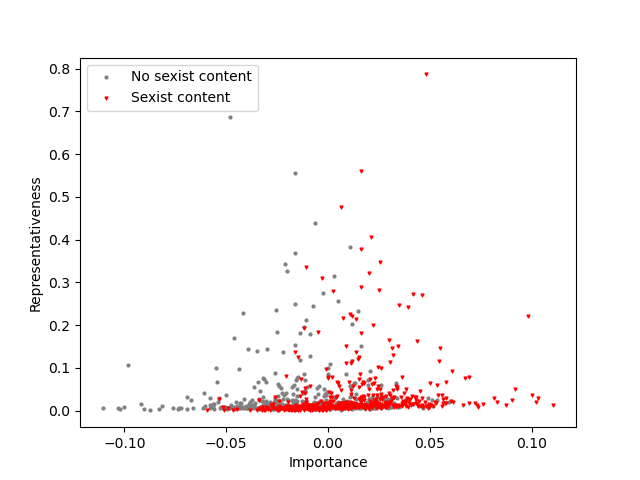
\includegraphics[width=0.9\textwidth]{figures/4-tweets/importance-rep-all-mean-unscaled.png}
    \caption[Representativeness values by LIME importance scores for features in the Twitter data]{Representativeness values by LIME importance scores.}
    \label{fig:tweets-rep}
\end{figure}
\begin{figure}[htbp]
    \centering
    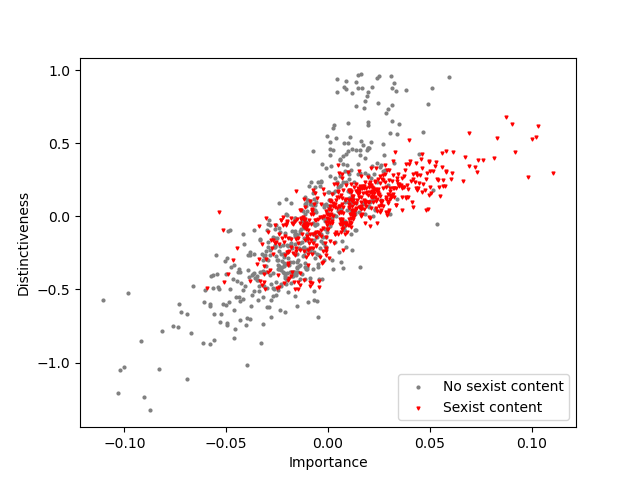
\includegraphics[width=0.9\textwidth]{figures/4-tweets/importance-dist-all-mean-unscaled.png}
    \caption[Distinctiveness values by LIME importance scores for features in the Twitter data]{Distinctiveness values by LIME importance scores.}
    \label{fig:tweets-dist}
\end{figure}

As with the dialect experiment, the importance scores and representativeness scores are (almost) independent of one another (\autoref{fig:tweets-rep}).
The correlation efficient between the two scores is 0.03 for importance values both for tweets with and without sexist content.
Most features that appear especially often in either of the tweet types have importance scores that are close to zero.

By contrast, as \autoref{fig:tweets-dist} shows, the distinctiveness scores and the LIME importance values show a clear correlation: the higher the importance score of a feature is for a given label, the more specific it is to samples with that (gold standard) label.
For both labels, the correlation coefficient for importance and distinctiveness is 0.8.
Importance scores for the group of tweets with sexist content are generally slightly higher than those for features in non-sexist tweets (see also \autoref{fig:tweets-dist}).

\begin{table}[htbp]
    \centering
\begin{tabular}{llrlrl}
\toprule
& & \multicolumn{2}{l}{\textbf{Sexist content}} & \multicolumn{2}{l}{\textbf{No sexist content}} \\
\midrule
{\hashtag} && {\cellcolor[HTML]{92D3B3}0.07} & {\hashtag} & {\cellcolor[HTML]{EEA8A3}-0.07} & {\hashtag} \\
{\hashtag} && {\cellcolor[HTML]{92D3B3}0.07} & {\hashtag} & {\cellcolor[HTML]{EEA8A3}-0.07} & {\hashtag} \\
ou & `or' &  &  &  &  \\
le & `the' &  &  &  &  \\
retour & `return' &  &  &  &  \\
des & `of the' &  &  &  &  \\
" & &{\cellcolor[HTML]{91D3B3}0.07} & \ngram{"\eow} & {\cellcolor[HTML]{EEA8A3}-0.07} & \ngram{"\eow} \\
pater && {\cellcolor[HTML]{A5DBC1}0.05} & \ngram{pa\mow} & {\cellcolor[HTML]{F2BAB6}-0.05} & \ngram{pa\mow} \\
familias &  &  &  &  \\
" && {\cellcolor[HTML]{91D3B3}0.07} & \ngram{"\eow} & {\cellcolor[HTML]{EEA8A3}-0.07} & \ngram{"\eow} \\
autant  & `as much as' & {\cellcolor[HTML]{F2BAB6}-0.05} & \ngram{autant\eow} & {\cellcolor[HTML]{ABDDC5}0.05} & \ngram{autant\eow} \\
dire  & `saying'&  &  &  &  \\
la & `the' &  &  &  &  \\
négation  & `negation'&  &  &  &  \\
radicale & `radical' &  &  &  &  \\
du & `of the' &  &  &  &  \\
féminisme  & `feminism'& {\cellcolor[HTML]{57BB8A}0.11} & \ngram{féminisme\eow{}} & {\cellcolor[HTML]{E67C73}-0.11} & \ngram{féminisme\eow{}} \\
par & `by' &  &  &  &  \\
ces & `these' & {\cellcolor[HTML]{ABDDC5}0.05} & \ngram{ces\eow{}} & {\cellcolor[HTML]{F1B8B3}-0.05} & \ngram{ces\eow{}} \\
spécialistes & `specialists' &  &  &  &  \\
de & `of' &  &  &  &  \\
l' & `the' &  &  &  &  \\
égalité  & `equality'& {\cellcolor[HTML]{5EBE8F}0.10} & \ngram{égalité\eow{}} & {\cellcolor[HTML]{E68078}-0.10} & \ngram{égalité\eow{}} \\
\bottomrule
\end{tabular}
    \caption[Local importance scores for a sample tweet]
    {Local importance scores for a sample tweet.
    Features with importance scores between -0.05 and +0.05 are omitted to preserve space.
    (Continued in the following table.)}
    \label{tab:results-tweets-sample-1}
\end{table}
\begin{table}[htbp]
    \centering
\begin{tabular}{llrlrl}
\toprule
& & \multicolumn{2}{l}{\textbf{Sexist content}} & \multicolumn{2}{l}{\textbf{No sexist content}} \\
\midrule
femme & `woman' & {\cellcolor[HTML]{57BB8A}0.11} & \ngram{femme\eow{}} & {\cellcolor[HTML]{E67C73}-0.11} & \ngram{femme\eow{}} \\
- &  &  &  &  \\
homme  & `man'& {\cellcolor[HTML]{7DCBA5}0.08} & \ngram{homme\eow{}} & {\cellcolor[HTML]{EB9992}-0.08} & \ngram{homme\eow{}} \\
, &  &  &  &  \\
qu' & `what' &  &  &  &  \\
en & `of it' &  &  &  &  \\
pense & `thinks' &  &  &  &  \\
Marlène &  &  &  &  \\
Schiappa &  &  &  &  \\
? &  &  &  & \\
\bottomrule
\end{tabular}
    \caption[Local importance scores for a sample tweet (continued)]
    {(Continuation of the previous table.)
    Local importance scores for a sample tweet.
    Features with importance scores between -0.05 and +0.05 are omitted to preserve space.}
    \label{tab:results-tweets-sample-2}
\end{table}

Tables~\ref{tab:results-tweets-sample-1} and~\ref{tab:results-tweets-sample-2} show the local importance scores for the tweet from Example~\ref{gloss:tweet-preprocessing}.
Since this is a binary classification task, each feature has the same absolute importance scores for both labels---only the sign is inverted.

\begin{figure}[htbp]
    \centering
    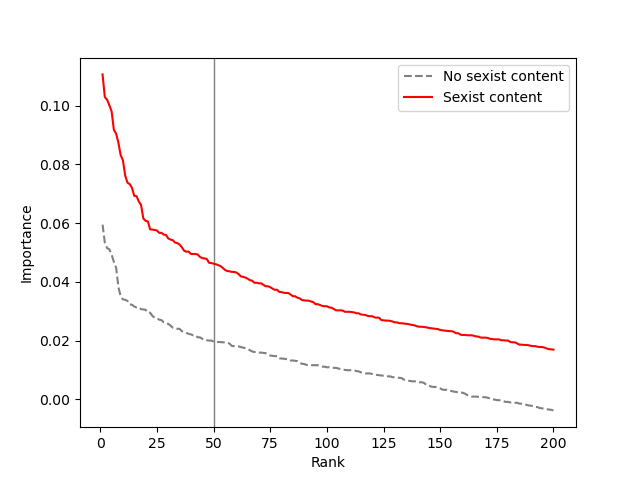
\includegraphics[width=0.9\textwidth]{figures/4-tweets/importance-rank-all-mean-unscaled-50.png}
    \caption[Importance scores for the 200 highest-ranking tweets per label]{Importance scores for the 200 highest-ranking tweets per label.}
    \label{fig:tweets-ranks}
\end{figure}

In the following, I examine patterns into which the top 50 most important features per label fit.
This cut-off point was also chosen to include most of the features with comparatively high importance scores while still retaining a large enough group in order to find patterns within this sub-selection.
\autoref{fig:tweets-ranks} shows the importance scores for the highest-ranking features in both label classes.
The 200 highest-ranking features per class can be found at \url{https://github.com/verenablaschke/ma-thesis/tree/main/models/tweets}.


\subsubsection{Words relating to gender}

\begin{table}[htbp]
    \centering
\begin{tabular}{llrrrl}
\toprule
\textbf{Group} & \textbf{Feature} & \multicolumn{1}{l}{\textbf{Imp.}} & \multicolumn{1}{l}{\textbf{Rep.}} & \multicolumn{1}{l}{\textbf{Dist.}} & \textbf{LIME?} \\
\midrule
\multirow{10}{*}{\begin{tabular}[c]{@{}l@{}}Sexist\\ content\end{tabular}} & \ngram{filles} `girls' & 0.20 & 0.02 & 0.55 &  \ngram{filles\eow}\\
 & \ngram{sexes} `sexes' & 0.20 & 0.01 & 0.39 &  \\
 & \ngram{femmes} `women' & 0.19 & 0.12 & 0.20 &  \ngram{femmes\eow}\\
 & \ngram{sexe} `sex' & 0.16 & 0.01 & 0.18 &  \\
 & \ngram{garçons} `boys'& 0.12 & 0.01 & 0.60 &  \\
 & \ngram{dame} `lady' & 0.10 & 0.00 & 0.02 & \\
 & \ngram{féminin} `feminine, female' & 0.09 & 0.01 & 0.07 & \\
 & \ngram{mecs} `guys' & 0.09 & 0.01 & 0.74 & \\
 & \ngram{fille} `girl' & 0.09 & 0.03 & 0.03 & \ngram{fille\eow}\\
 & \ngram{femme} `woman' & 0.09 & 0.23 & 0.26 & \ngram{femme\eow}\\
 \bottomrule
\end{tabular}
    \caption
    [Features with the top 50 highest LIME scores per label relating to gender]
    {Features with the top 50 highest LIME scores per label that are related to gender.
    The middle columns contain importance, representativeness and distinctiveness scores.
    The context column lists the most frequent word in which each token appears (along with the relative frequency of this word being the origin).
    }
    \label{tab:gender-words}
\end{table}

Many of the tokens that appear in tweets with sexist content and that have high importance scores relate to gender in some way (\autoref{tab:gender-words}).
Most of these are words or subtokens of words that describe women (\textit{filles} `girls,' \textit{femme(s)} `woman/women,' \textit{meuf(s)} `woman/women (colloq.)' and \textit{elles} `they.\textsc{fem}'),\footnote{%
The latter does not always refer to groups of women, it substitutes any plural noun phrase that is grammatically feminine.}
although two words for men also make it into the top 50 (\textit{homme} `man,' \textit{mec} `guy').
Notably, the class of tweets without sexist content also contains one high-importance token referring to women, which is the singular form of one of the aforementioned features: \textit{fille} `girl.' 
However, this word actually appears marginally less often in tweets with this label as one would a randomly distributed feature expect to appear.

\subsubsection{Words relating to feminism and sexism}

\begin{table}[htbp]
    \centering
\begin{tabular}{llrrrl}
\toprule
\textbf{Label} & \textbf{Feature} & {\textbf{Imp.}} & {\textbf{Rep.}} & {\textbf{Dist.}} & \textbf{Context} \\
\midrule
\multirow{4}{*}{\begin{tabular}[c]{@{}l@{}}Sexist\\ content\end{tabular}} & \ngram{féminisme\eow} & 0.11 & 0.01 & 0.30 & féminisme(1.0) `feminism' \\
 & \ngram{égalité\eow} & 0.08 & 0.03 & 0.40 & égalité(1.0) `equality'\\
 & \ngram{sexiste\eow} & 0.06 & 0.02 & 0.25 & sexiste(1.0) `sexist' \\
 & \ngram{féministe\eow} & 0.06 & 0.03 & 0.21 & féministe(1.0) `feminist'\\
 \midrule
\begin{tabular}[c]{@{}l@{}}No sexist\\ content\end{tabular} & \ngram{sexisme\eow} & 0.03 & 0.06 & 0.35 & sexisme(1.0) `sexism'\\
\bottomrule
\end{tabular}
    \caption
    [Features with the top 50 highest LIME scores per label relating to feminism or sexism]
    {Features with the top 50 highest LIME scores per label that are directly related to feminism or sexism.
    The middle columns contain importance, representativeness and distinctiveness scores.
    The context column lists the most frequent word in which each token appears (along with the relative frequency of this word being the origin).
    }
    \label{tab:feminism-sexism}
\end{table}

Several of the features with high importance scores are connected to discussions of feminism or sexism.
Here, tokens relating to feminism or equality are indicators of tweets with sexist content, while the features mentioning sexism are split: \ngram{sexiste\eow} `sexist' is an indicator for sexist content whereas \ngram{sexisme\eow} `sexism' has a high importance score for tweets with \textit{no} sexist content (\autoref{tab:feminism-sexism}).

\subsubsection{Gendered insults}

\begin{table}[htbp]
    \begin{tabular}{llrrrl}
\toprule
\textbf{Label} & \textbf{Feature} & \multicolumn{1}{l}{\textbf{Imp.}} & \multicolumn{1}{l}{\textbf{Rep.}} & \multicolumn{1}{l}{\textbf{Dist.}} & \textbf{Context} \\
\midrule
\multirow{2}{*}{Sexist content} & \ngram{salope\eow} & 0.08 & 0.02 & 0.53 & salope(1.0) `slut, bitch' \\
 & \ngram{asse\eow} & 0.08 & 0.02 & 0.38 & connasse(0.8) `bitch' \\
 \midrule
No sexist content & \ngram{conne\eow} & 0.03 & 0.01 & 0.02 & conne(1.0) `stupid.\textsc{fem}'\\
\bottomrule
\end{tabular}
    \caption
    [Features with the top 50 highest LIME scores per label that are gendered insults]
    {Features with the top 50 highest LIME scores per label that are (subtokens) of insults directed at women.
    The middle columns contain importance, representativeness and distinctiveness scores.
    The context column lists the most frequent word in which each token appears (along with the relative frequency of this word being the origin).
    }
    \label{tab:insults}
\end{table}


Two of the high-ranking features of tweets with sexist contents are (subtokens of) insults directed at women: \ngram{salope\eow} `slut, bitch' and \ngram{asse\eow}, which almost always appears as the suffix of \textit{connasse} `bitch' in this dataset.
However, one of the top 50 indicators of a non-sexist tweet is also such a term: \textit{conne} `bitch; stupid.\textsc{fem}'
Both of the features with high importance scores for the sexist class have high distinctiveness scores, whereas \textit{conne} only occurs in the tweets without sexist content roughly as often as one would expect by chance (see \autoref{tab:insults}).

The presence of insults that either relate to intellectual deficits or that pertain to sexuality fits with the observations that \citet{dupre2020violences} made in a qualitative analysis of sexist tweets.

\subsubsection{Female politicians}

\begin{table}[htbp]
    \centering
\begin{tabular}{llrrrl}
\toprule
\textbf{Label} & \textbf{Feature} & \multicolumn{1}{l}{\textbf{Imp.}} & \multicolumn{1}{l}{\textbf{Rep.}} & \multicolumn{1}{l}{\textbf{Dist.}} & \textbf{Context} \\
\midrule
\multirow{9}{*}{\begin{tabular}[c]{@{}l@{}}No sexist\\ content\end{tabular}} & \ngram{Ségolène\eow} & 0.05 & 0.03 & 0.88 & Ségolène(1.0)  \\
 & \ngram{Christiane\eow} & 0.05 & 0.03 & 0.77 & Christiane(1.0)  \\
 & \ngram{Royal\eow} & 0.04 & 0.03 & 0.87 & Royal(1.0)  \\
 & \ngram{Angela\eow} & 0.03 & 0.06 & 0.86 & Angela(1.0)  \\
 & \ngram{Theresa\eow} & 0.03 & 0.03 & 0.91 & Theresa(1.0)  \\
 & \ngram{Christine\eow} & 0.03 & 0.02 & 0.77 & Christine(1.0)  \\
 & \ngram{Taubira\eow} & 0.03 & 0.03 & 0.74 & Taubira(1.0)  \\
 & \ngram{Lagarde\eow} & 0.02 & 0.01 & 0.78 & Lagarde(1.0)  \\
 & \ngram{May\eow} & 0.02 & 0.03 & 0.89 & May(1.0) \\
 \bottomrule
\end{tabular}
    \caption
    [Features with the top 50 highest LIME scores per label that are names of female politicians]
    {Features with the top 50 highest LIME scores per label that are names of female politicians.
    The middle columns contain importance, representativeness and distinctiveness scores.
    The context column lists the most frequent word in which each token appears (along with the relative frequency of this word being the origin).
    }
    \label{tab:politicians}
\end{table}

Many of the features with high importance scores for the tweets without sexist content are the first and last names of several influential female politicians (Ségolène Royal, Christiane Taubira, Christine Lagarde, Angela Merkel and Theresa May).
While none of these names appear in an especially high proportion of the non-sexist tweets, all them them appear almost exclusively in this class (\autoref{tab:politicians}).

\subsubsection{Pronouns}

\begin{table}[htbp]
    \centering
\begin{tabular}{llrrrl}
\toprule
\textbf{Label} & \textbf{Feature} & \multicolumn{1}{l}{\textbf{Imp.}} & \multicolumn{1}{l}{\textbf{Rep.}} & \multicolumn{1}{l}{\textbf{Dist.}} & \textbf{Context} \\
\midrule
\multirow{10}{*}{\begin{tabular}[c]{@{}l@{}}Sexist\\ content\end{tabular}} & \ngram{t'\eow} & 0.10 & 0.04 & 0.53 & t'(1.0) `your.\textsc{sg}' \\
 & \ngram{te\eow} & 0.09 & 0.05 & 0.44 & te(0.8)  `you.\textsc{sg.acc}'\\
 & \ngram{ta\eow} & 0.06 & 0.02 & 0.26 & ta(0.9) `your.\textsc{sg}'  \\
 & \ngram{tes\eow} & 0.06 & 0.02 & 0.45 & tes(0.6) `your.\textsc{sg}'  \\
 & \ngram{ton\eow} & 0.06 & 0.03 & 0.31 & ton(1.0) `your.\textsc{sg}'  \\
 & \ngram{me\eow} & 0.06 & 0.07 & 0.31 & me(0.9) `me'  \\
 & \ngram{moi\eow} & 0.06 & 0.04 & 0.34 & moi(1.0) `I, me' \\
 & \ngram{ma\eow} & 0.05 & 0.04 & 0.25 & ma(1.0) `my' \\
 & \ngram{toi\eow} & 0.05 & 0.02 & 0.37 & toi(1.0) `you' \\
 & \ngram{mes\eow} & 0.05 & 0.01 & 0.16 & mes(0.9) `my'\\
 \bottomrule
\end{tabular}
    \caption
    [Features with the top 50 highest LIME scores per label that are personal pronouns]
    {Features with the top 50 highest LIME scores per label that are personal pronouns.
    The middle columns contain importance, representativeness and distinctiveness scores.
    The context column lists the most frequent word in which each token appears (along with the relative frequency of this word being the origin).
    }
    \label{tab:tweets-pronouns}
\end{table}

As \autoref{tab:tweets-pronouns} shows, ten of the 50 features with the highest importance scores for the tweets with sexist contents are first and second person singular (informal) pronouns, and these features do indeed also have high distinctiveness scores for that class.
No personal pronouns are included in the top 50 features for the other label.
The fact that so many first and second person pronouns are indicators for sexist content fits the definition of two of the subcategories within that class in the corpus: tweets with sexist content that is \textit{directed} at someone often include second person pronouns by their nature, and tweets \textit{reporting} encounters with sexism often contain first person pronouns (or second person pronouns, if they include direct quotations).

\subsubsection{Punctuation}

Four of the features that LIME deems indicative of sexist content consist of punctuation marks (\ngram{—\eow}, \ngram{...\eow}, \ngram{=\eow} and \ngram{?\mow}), as does one of the high-ranking features of the other class (\ngram{,\mow}).\footnote{%
This should not be confused with the more common comma feature \ngram{,\eow}.
The above-mentioned feature is much rarer and appears in character sequences such as \textit{,''} where it is followed by other letters (usually other punctuation marks).
}
% Of these, the em-dash has the highest distinctiveness score  (0.62), although it is not obvious...

\newpage
\section{Attention}
\label{sec:tweets-method-attn}

\subsection{Preprocessing and method}

I lowercase the tweets and embed them using pretrained word2vec \citep{mikolov2013distributed} embeddings for French, as provided by \citet{fares2017word}.\footnote{%
They can be downloaded via \url{http://vectors.nlpl.eu/repository/20/43.zip}.}
These embeddings work on a word (and punctuation) level rather than a sub-token level.
I truncate all tweets that are longer than sixty tokens (that is, words or (clusters of) punctuation marks) and pad all shorter tweets with dummy tokens (\ngram\filler).


I use a feed-forward neural network with an attention layer, as illustrated in \autoref{sec:attention-what}.
In preliminary experiments, the choice between an FFNN and a recurrent neural network did not lead to significant differences in the classification accuracy.
I therefore use the FFNN since the hidden representations produced by a recurrent model might be less directly reflective of the individual input tokens.
I use a hidden layer size of 128 for the FFNN, a dropout rate of 0.4 between the FFNN and the attention layer, and train the model with a batch size of 64 and a learning rate of 0.01 with an Adam optimizer.
To build and train the model, I use the Python library Keras\footnote{\url{https://keras.io}} 2.4.3 with a Tensorflow\footnote{\url{https://www.tensorflow.org/}} 2.4.1 backend.

As with the other experiments, all metrics and scores are averaged across ten initializations and train-test splits.

\subsection{Results}
\label{sec:tweets-attn-results}

The neural classifiers have an average accuracy of 73.9~\% and F$_1$ score of 72.5~\% across the ten initializations.%
\footnote{These scores cannot be directly compared to the classifier performances that \citet{chiril2020annotated} report for the same dataset, since their test set has a different label distribution than mine.
The test sets I work with all have a label ratio of approximately 1:2 (sexist content vs. non-sexist content), whereas \citeauthor{chiril2020annotated} use a more balanced ratio of circa 3:5.
That said, their neural, non-BERT models achieve accuracy scores of up to 69.5~\% and F$_1$ scores of up to 64.0~\%.
Their best model is a mulitilingual BERT model \citep{devlin2019bert} with a classification layer that has an accuracy of 79.0~\% and an F$_1$ score of 76.2~\%.}

I extract attention weights for tokens in the test sets and discard those that appear less than twenty times.
I then calculate the global attention score for each token by averaging the attention weights that the token is associated with in the different tweets and initializations.
The highest global attention score is 0.27.

I also examine the distribution of the attention weights per utterance.
On average, the entropy of the attention weight distribution for a tweet is 2.58, with a standard deviation of 1.24.
For comparison, the maximum possible entropy for a probability distribution with 60 possible outcomes is 4.09.
Some tweets have attention weight vectors that are very nearly one-hot encoded (with an entropy of 0.0001), i.e. where the attention lies very clearly on a single token, whereas some others have uniform attention distributions (with an entropy of 4.09), but most lie somewhere in the middle.

The {\ngram\filler} tokens have a mean attention weight of 0.01, i.e. an attention score that is only marginally higher than the weight of 0 one might expect.


\begin{figure}[htbp]
    \centering
    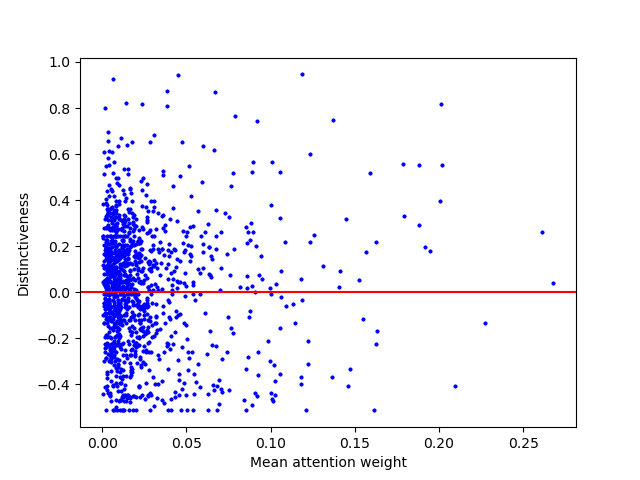
\includegraphics[width=0.9\textwidth]{figures/3-dialects/attention-distinctiveness.png}
    \caption[Distinctiveness values by attention weight for features in the Twitter data]{Distinctiveness values by global attention weight.}
    \label{fig:attn-dist}
\end{figure}

\autoref{fig:attn-dist} shows the global attention weights as well as the corresponding distinctiveness scores.
The latter are calculated with regard to the class of tweets with sexist content.
Positive distinctiveness scores indicate that a feature appears especially often in sexist tweets (the upper bound is 1.0) and negative scores indicate that a feature occurs especially often in non-sexist tweets (with a lower bound of -0.51).
Unlike in the LIME experiments, there is no significant correlation between the attention(/importance) score a feature has and how distinctive it is: many features that are very characteristic of one class of tweets have low attention weights, and some of the features with high global attention scores have distinctiveness values close to zero.
For instance, the feature with the highest attention score, \ngram{pourrait} `could,' has a distinctiveness score of only 0.04.

In the following section, I consider the 100 tokens with the highest global attention weights (this represents a range of attention scores from 0.08 to 0.27) and compare recurrent types of tokens present in that group to those present in the LIME results (\autoref{sec:tweets-svm-results}).
The full list of attention weights is available at \url{https://github.com/verenablaschke/ma-thesis/tree/main/models/tweets-attn}.

The attention weights are not label-specific---a high attention weight only means that the FFNN-encoded representation of a token receives a greater weight when making the final classification decision.
I therefore consider all (high-attention) features with positive distinctiveness scores to be indicators of sexist content, and features with negative distinctiveness scores to be important predictors for tweets with no sexist content.

% \subsection{Recurring feature types}

\subsubsection{Words relating to gender or sex}
\begin{table}[htbp]
    \centering
\begin{tabular}{llrrrl}
\toprule
\textbf{Group} & \textbf{Feature} & \multicolumn{1}{l}{\textbf{Imp.}} & \multicolumn{1}{l}{\textbf{Rep.}} & \multicolumn{1}{l}{\textbf{Dist.}} & \textbf{LIME?} \\
\midrule
\multirow{10}{*}{\begin{tabular}[c]{@{}l@{}}Sexist\\ content\end{tabular}} & \ngram{filles} `girls' & 0.20 & 0.02 & 0.55 &  \ngram{filles\eow}\\
 & \ngram{sexes} `sexes' & 0.20 & 0.01 & 0.39 &  \\
 & \ngram{femmes} `women' & 0.19 & 0.12 & 0.20 &  \ngram{femmes\eow}\\
 & \ngram{sexe} `sex' & 0.16 & 0.01 & 0.18 &  \\
 & \ngram{garçons} `boys'& 0.12 & 0.01 & 0.60 &  \\
 & \ngram{dame} `lady' & 0.10 & 0.00 & 0.02 & \\
 & \ngram{féminin} `feminine, female' & 0.09 & 0.01 & 0.07 & \\
 & \ngram{mecs} `guys' & 0.09 & 0.01 & 0.74 & \\
 & \ngram{fille} `girl' & 0.09 & 0.03 & 0.03 & \ngram{fille\eow}\\
 & \ngram{femme} `woman' & 0.09 & 0.23 & 0.26 & \ngram{femme\eow}\\
 \bottomrule
\end{tabular}
    \caption
    [Features with the top 100 highest attention scores relating to gender or sex]
    {Features with the top 100 highest attention scores relating to gender or sex.
    The middle columns contain importance, representativeness and distinctiveness\protect\footnotemark{} scores.
    The right-most column lists the corresponding features presented in \autoref{sec:tweets-svm-results}, if applicable.
    }
    \label{tab:attn-gender}
\end{table}
\footnotetext{Some of the distinctiveness scores deviate slightly from the corresponding ones in the LIME results due to the different tokenization approaches.}

Several of the words with high attention scores relate to gender or sex.
They are shown in \autoref{tab:attn-gender}.
Notably, all of these tend to occur especially often in tweets with sexist content (with the exception of \textit{dame} `lady,' which has a distinctiveness score that is barely above 0).
There is some overlap between this group and the gender-related words among the tokens with high LIME importance scores, but many of these terms appear only in the results of one experiment but not the other.
These differences \textit{cannot} be explained because of the vocabulary of the word2vec embeddings, since these also contain more colloquial terms like \textit{meuf} `woman' (which has a high LIME score).

\subsubsection{Words relating to feminism and sexism}
\begin{table}[htbp]
    \centering
\begin{tabular}{llrrrl}
\toprule
\textbf{Label} & \textbf{Feature} & {\textbf{Imp.}} & {\textbf{Rep.}} & {\textbf{Dist.}} & \textbf{Context} \\
\midrule
\multirow{4}{*}{\begin{tabular}[c]{@{}l@{}}Sexist\\ content\end{tabular}} & \ngram{féminisme\eow} & 0.11 & 0.01 & 0.30 & féminisme(1.0) `feminism' \\
 & \ngram{égalité\eow} & 0.08 & 0.03 & 0.40 & égalité(1.0) `equality'\\
 & \ngram{sexiste\eow} & 0.06 & 0.02 & 0.25 & sexiste(1.0) `sexist' \\
 & \ngram{féministe\eow} & 0.06 & 0.03 & 0.21 & féministe(1.0) `feminist'\\
 \midrule
\begin{tabular}[c]{@{}l@{}}No sexist\\ content\end{tabular} & \ngram{sexisme\eow} & 0.03 & 0.06 & 0.35 & sexisme(1.0) `sexism'\\
\bottomrule
\end{tabular}
    \caption
    [Features with the top 100 highest attention scores relating to feminism or sexism]
    {Features with the top 100 highest attention scores relating to feminism or sexism.
    The middle columns contain importance, representativeness and distinctiveness scores.
    The right-most column lists the corresponding features presented in \autoref{sec:tweets-svm-results}, if applicable.
    }
    \label{tab:attn-feminism}
\end{table}

As in the LIME results, many high-ranking words are directly related to feminism or sexism (\autoref{tab:attn-feminism}).
The corresponding features with high attention weights contain all of the feminism/sexism-related tokens with high LIME importance scores, as well as one additional term (\textit{parité} `parity').

\subsubsection{Gendered insults}

Three of the tokens with high attention weights are insults directed at women: \textit{connasse} `bitch' and \textit{salope} `slut, bitch' (both of which have (subtokens that have) high LIME importance scores for the class of sexist tweets) and \textit{pute} `whore' (which---unsurprisingly---almost exclusively appears in tweets with sexist content, but is not among the 50 features with the highest LIME importance scores for that class).

\subsubsection{Female politicians}
\begin{table}[htbp]
    \centering
\begin{tabular}{llrrrl}
\toprule
\textbf{Label} & \textbf{Feature} & \multicolumn{1}{l}{\textbf{Imp.}} & \multicolumn{1}{l}{\textbf{Rep.}} & \multicolumn{1}{l}{\textbf{Dist.}} & \textbf{Context} \\
\midrule
\multirow{9}{*}{\begin{tabular}[c]{@{}l@{}}No sexist\\ content\end{tabular}} & \ngram{Ségolène\eow} & 0.05 & 0.03 & 0.88 & Ségolène(1.0)  \\
 & \ngram{Christiane\eow} & 0.05 & 0.03 & 0.77 & Christiane(1.0)  \\
 & \ngram{Royal\eow} & 0.04 & 0.03 & 0.87 & Royal(1.0)  \\
 & \ngram{Angela\eow} & 0.03 & 0.06 & 0.86 & Angela(1.0)  \\
 & \ngram{Theresa\eow} & 0.03 & 0.03 & 0.91 & Theresa(1.0)  \\
 & \ngram{Christine\eow} & 0.03 & 0.02 & 0.77 & Christine(1.0)  \\
 & \ngram{Taubira\eow} & 0.03 & 0.03 & 0.74 & Taubira(1.0)  \\
 & \ngram{Lagarde\eow} & 0.02 & 0.01 & 0.78 & Lagarde(1.0)  \\
 & \ngram{May\eow} & 0.02 & 0.03 & 0.89 & May(1.0) \\
 \bottomrule
\end{tabular}
    \caption
    [Features with the top 100 highest attention scores relating to female politicians]
    {Features with the top 100 highest attention scores relating to female politicians.
    The middle columns contain importance, representativeness and distinctiveness scores.
    The right-most column lists the corresponding features presented in \autoref{sec:tweets-svm-results}, if applicable.
    }
    \label{tab:attn-politicians}
\end{table}

Similarly to the LIME results, several tokens with high attention scores refer to female politicians.
There is only partial overlap between the two experiments' results however, and the attention-based results also include (female) job titles in addition to names of politicians (\autoref{tab:attn-gender}).
With the exception of the last name of Marlène Schiappa (who used to be the French Secretary of State for Gender Equality), all of these tokens mostly appear in tweets without sexist content. 

\subsubsection{Pronouns and punctuation}

Unlike the results of the LIME experiment, none of the high-ranking tokens are personal pronouns or contain punctuation marks.

\subsubsection{Body parts}
\begin{table}[htbp]
    \centering
\begin{tabular}{llrrrl}
\toprule
\textbf{Group} & \textbf{Feature} & \multicolumn{1}{l}{\textbf{Imp.}} & \multicolumn{1}{l}{\textbf{Rep.}} & \multicolumn{1}{l}{\textbf{Dist.}} & \textbf{LIME?} \\
\midrule
\multirow{3}{*}{\begin{tabular}[c]{@{}l@{}}Sexist\\ content\end{tabular}} & \ngram{seins} `breasts' & 0.20 & 0.01 & 0.82 &  \\
 & \ngram{bite} `dick' & 0.14 & 0.01 & 0.75 &  \\
 & \ngram{fesses} `buttocks' & 0.08 & 0.01 & 0.77 & \\
 \bottomrule
\end{tabular}
    \caption
    [Features with the top 100 highest attention scores describing body parts]
    {Features with the top 100 highest attention scores describing body parts.
    The middle columns contain importance, representativeness and distinctiveness scores.
    The right-most column lists the corresponding features presented in \autoref{sec:tweets-svm-results}, if applicable.
    }
    \label{tab:attn-body}
\end{table}

Three of the tokens with high global attention weights refer to body parts, as shown in \autoref{tab:attn-body}.
All of these words mostly appear in tweets with sexist content, and none of them are among the tokens with the highest LIME importance scores.

\newpage
\subsection{Discussion}
\label{sec:dialects-discussion}

Many of the features that got assigned high importance scores by LIME serve as examples for the linguistic patterns described by dialectologists.
However, not all features that are important for the label prediction are easy to understand for humans or fall into easily recognizable feature categories.
Additionally, many of the features with high-importance scores showcase linguistic traits that are not often discussed in Norwegian dialectology, such as the different variants of \textit{noe(n)} `some, somebody, something' or the past participle endings in North Norwegian.

The features that have high importance scores for a dialect group are not always very representative of the entire group (although these exist, such as the West Norwegian /(r)rs/), but sometimes only represent characteristic traits of the dialects spoken in one subregion (e.g. the diphthongs /ao, \aa{}o/ in some parts of West Norway).
This also results in there sometimes being several seemingly contradictory features that have high importance scores for the same label, such as the West Norwegian first person singular variants /i/, /ei/ and /eg/ that are all among the 50 highest-ranking features for that dialect group.
It would be interesting to explore how this might change if the number of input features is restricted further and relatively infrequent features are excluded.

It might also be insightful to examine the importance scores for features that are encoded differently, for instance as sound correspondences between the dialects and a reference doculect.

Furthermore, it would be worthwhile to explore which features have high importance scores and are common in false positives/negatives: are there patterns as to which linguistic features lead the classifier astray?


\chapter{Conclusion} 
\label{chap:conclusion}

Both in a traditional linguistic context such as dialectology and in a more recent applied context such as detecting sexist content in tweets, applying explainable machine learning techniques can be insightful.
In both tasks, many of the features with high importance scores fall into recurring groups that can be analyzed.
In the case of dialect classification, some of these groups fit in with common dialectological observations while others present patterns in the data that are not typically discussed.
In the context of tweet classification, these groups of features can be used to determine whether a model is trustworthy enough to be used in real applications.
While the attention weights for input features produce somewhat similar high-ranking results as LIME does, they fail at putting particular focus on highly distinctive features and thus produce less trustworthy insights into the model's classification process.

There is ample opportunity for continuing this work, for instance by exploring which input features with high importance scores tend to appear in incorrectly classified utterances or tweets, or by applying other kinds of explainable machine learning and comparing the results.



% \editnotesummary

\bibliography{bib/dialect-data,bib/dialectology,bib/dialectometry,bib/explainable-ml,bib/tweets}

\end{document}
